\chapter{Direct backward ray mapping}
\label{chap:raymapping2}
In Chapter \ref{chap:raymapping1} we introduced an inverse method based on ray mapping reconstruction in PS.
The goal was to calculate the intensity distribution at the target of an optical system. \\ \indent
The idea was to construct a map from the target \point{T} to the source \point{S} using the PS of all the optical lines, which are divided into several regions.  
The method developed in the previous chapter requires that the boundaries of these regions can be determined exactly in every PS. Therefore, also the positive luminance regions were found analytically and the \textit{exact} intensity could be determined. This is only possible for systems formed by straight line segments.\\ \indent
In this chapter we modify the method to systems formed by curved lines. In this case, the boundaries of the regions in PS cannot be determined exactly.
Because of this, we need to apply a numerical procedure. In particular, we develop a method that employs only the PS of the target of the system. 
% Differences
The boundaries are detected applying a bisection procedure in target PS in combination with backward ray tracing. The method is tested for two optical systems: the TIR-collimator and a parabolic reflector. The results are presented in Section \ref{sec:TIR} and \ref{sec:PR}, respectively.
\section{Bisection method and backward ray tracing}\label{sec:raymapping_explanation}
The purpose of this section is to present the modified backward ray mapping method valid for systems formed by curved lines. 
Given a partition $P: -1 = \variabile{p}^0<\variabile{p}^1<\cdots<\variabile{p}^{\nbin}=1$ of the interval $[-1,1]$ with $\nbin$ the number of bins in the partitioning, the intensity in target PS is given by Equation (\ref{eta2}) for every $\dir{}{}\in P$.
Therefore, the problem reduces to calculating the coordinates 
$\variabile{q}^{\textrm{\,min}}(\Pi, \variabile{p})$ and $\variabile{q}^{\textrm{\,max}}(\Pi, \variabile{p})$ of the rays on $\partial$\set{R}{}{}$(\Pi)$ for every path $\Pi$. 
\\ \indent 
We indicate with $(\variabile{q}^{\,\textrm{a}}, \variabile{p})= (-\variabile{b}, \variabile{p})$ and $(\variabile{q}^{\,\textrm{b}}, \variabile{p}) = (\variabile{b}, \variabile{p})$ the coordinates of the end points of \set{T}{}{} along direction $\variabile{p}$. These points are associated to two rays in PS. Consider the corresponding position coordinate $(\variabile{x}^{\textrm{a}}, \variabile{z}^{\textrm{a}})$ and $(\variabile{x}^{\textrm{b}}, \variabile{z}^{\textrm{b}})$ and angular coordinates $\optangle^{\variabile{a}}$ and $\optangle^{\variabile{b}}$ of the ray in real space, where $\variabile{x}^{\textrm{a}} = \variabile{q}^{\textrm{a}}$, $\variabile{x}^{\textrm{b}} = \variabile{q}^{\textrm{b}}$, $\variabile{z}^{\textrm{a}} = \variabile{z}^{\textrm{b}} = \variabile{h}$ where $\variabile{h}$ is the height of the target and $\optangle^{\textrm{a}}= \optangle^{\textrm{b}}=\variabile{p}$ refers to the emitted ray. Next, the rays parametrizations $\vect{r}_{\textrm{a}}(s)$ and $\vect{r}_{\textrm{b}}(s)$ are determined according to (\ref{parametrization}).
We remind the reader that, in real space, the coordinates of each ray on line $\lineai\neq \nline$ are indicated with $(\variabile{x}_{\lineai}, \variabile{z}_{\lineai})$ and $\optangle_{\lineai}$ where $(\variabile{x}_{\lineai}, \variabile{z}_{\lineai})$ are the coordinate of the intersection point between the ray and line $\lineai$ and $\optangle_{\lineai}$ is the direction of the incident ray with respect to the \textit{optical axis}. 
%We remind the reader that in the previous chapter we indicated with $(\pos{t,}{\lineai},\dir{t,}{\lineai})$ the coordinates of the rays in target PS \set{T}{\lineai}{} in where the directions coordinates were expressed with respect to the \textit{normal} of line $\lineai$. Note that $\pos{\lineai}{}=\pos{t,}{\lineai}$ while $\dir{\lineai}{}\neq\dir{t,}{\lineai}$. We introduce the notation $(\pos{\lineai}{}^{\textrm{a}}, \dir{\lineai}{}^{\textrm{a}})$ for the coordinates of ray $\vect{r}_{\textrm{a}}(s)$ on line $\lineai$.\\ \indent 
The procedure starts with intensity $I(\variabile{p})=0$ and the end points $(\variabile{q}^{\,\textrm{a}}, \variabile{p})= (-\variabile{b}, \variabile{p})$ and $(\variabile{q}^{\,\textrm{b}}, \variabile{p}) = (\variabile{b}, \variabile{p})$. Since the boundaries of the regions in all the phase spaces are unknown, to determine from which line $\vect{r}_{\textrm{a}}$ and $\vect{r}_{\textrm{b}}$ are emitted we apply backward ray tracing. We denote with $\nline$ the index of the target (line $\nline$) and with $\lineaj\in\{1,\cdots, \nline-1\}$ and $\lineak\in\{1,\cdots, \nline-1\}$ the lines from which the rays with parametrization $\vect{r}_{\textrm{a}}(s)$ and $\vect{r}_{\textrm{b}}()$ are emitted, respectively. $\Pi^\textrm{a} = (\lineaj, \nline)$ and $\Pi^\textrm{b} = (\lineak,\nline)$ are the last part of the paths followed by the two rays $\vect{r}_{\textrm{a}}$ and $\vect{r}_{\textrm{b}}$, respectively. $(\variabile{q}^{\textrm{a}}, \variabile{p})\in\partial$\set{R}{}{}$(\Pi^{\textrm{a}})$ and $(\variabile{q}^{\textrm{b}}, \variabile{p})\in\partial$\set{R}{}{}$(\Pi^{\textrm{b}})$. At this stage we know whether the two rays are emitted from the same line or not. \\ \indent 
First, assume $\lineaj= \lineak$, then $\vect{r}_{\textrm{a}}$ and $\vect{r}_{\textrm{b}}$ hit the same line before reaching the target. 
In case $\lineaj = 1$ a possible path from the source to the target is found and, assuming a Lambertian source, the intensity is updated according to:
\begin{equation}\label{eq:intensity_brm}
I(\variabile{p}) = I(\variabile{p})+\variabile{q}^{\textrm{max}}(\Pi^\textrm{a}, \variabile{p})-\variabile{q}^{\textrm{min}}(\Pi^\textrm{a}, \variabile{p}),
\end{equation}
where $\variabile{q}^{\textrm{min}}(\Pi^\textrm{a}, \variabile{p}) = \variabile{q}^{\textrm{min}} = \min\{\variabile{q}^{\textrm{a}}, \variabile{q}^{\textrm{b}}\}$ and $\variabile{q}^{\textrm{max}}(\Pi^\textrm{a}, \variabile{p}) = \variabile{q}^{\textrm{max}} = \max\{\variabile{q}^{\textrm{a}}, \variabile{q}^{\textrm{b}}\}$. In case $\lineaj\neq 1$ the two rays $\vect{r}_{\textrm{a}}$ and $\vect{r}_{\textrm{b}}$ are traced back further using backward ray tracing.
\\ \indent Next, if $\lineaj\neq \lineak$ the rays $\vect{r}_\textrm{a}$ and $\vect{r}_\textrm{b}$ are emitted from two different lines, hence $\Pi^{\textrm{a}}\neq \Pi^{\textrm{b}}$ and belong to different regions \set{R}{}{}$(\Pi^{\textrm{a}})$ and \set{R}{}{}$(\Pi^{\textrm{b}})$ in \set{T}{}{}. $\variabile{q}^{\textrm{a}}$ in $\mbox{\set{R}{}{}}(\Pi^{\textrm{b}})$, the other intersection points of line 
$\variabile{p}=\textrm{const}$ with the boundary $\mbox{\set{R}{}{}}(\Pi^{\textrm{b}})$ are unknown. To determine the other coordinates of the rays on the boundary $\partial$\set{R}{}{}$(\Pi^{\textrm{a}})$, the bisection method is applied to the segment $[\variabile{q}^{\,\textrm{a}}(\Pi^{\textrm{a}}, \variabile{p}), \variabile{q}^{\,\textrm{b}}(\Pi^{\textrm{b}}, \variabile{p})]$ in target PS \set{T}{}{} along direction $\variabile{p}$. Thus, this interval is repeatedly halved until the position coordinate in target PS of the ray that follows the same path $\Pi^{\textrm{a}}$ of $\vect{r}_{\textrm{a}}$ is found (the corresponding direction coordinate $\variabile{p}$ is fixed). The bisection procedure continues until the length of the segment considered becomes smaller than a fixed tolerance. 
Giving as input the coordinates $\variabile{q}^{\,\textrm{a}}(\Pi^{\textrm{a}}, \variabile{p})$ and $\variabile{q}^{\,\textrm{b}}(\Pi^{\textrm{b}}, \variabile{p})$ of the rays with parametrization $\vect{r}_{\textrm{a}}(s)$ and $\vect{r}_{\textrm{b}}(s)$, the path $\Pi^\textrm{a}$ and the tolerance $\textrm{tol}= 10^{-12}$, the bisection method is implemented as in Algorithm \ref{alg:bisection}. Similarly, others paths will be obtained later using the same procedure applied to another interval in target PS.
\begin{algorithm}
\caption{Bisection($\variabile{q}^{\,\textrm{a}}(\Pi^{\textrm{a}}, \variabile{p})$, $\variabile{q}^{\,\textrm{b}}(\Pi^{\textrm{b}}, \variabile{p})$,$\vect{r}_{\textrm{a}}(s)$, $\vect{r}_{\textrm{b}}(s)$, \textrm{tol}, $\Pi^\textrm{a}$)}\label{alg:bisection}
Initialize: $\textrm{step} = 0$, $\lineai = \nline$
\begin{algorithmic}[1]
\While {$|\variabile{q}^{\,\textrm{a}}-\variabile{q}^{\,\textrm{b}}|>\textrm{tol}$}
\State $\variabile{x}_{\lineai}^{\textrm{m}}=\variabile{q}^{\,\textrm{m}}= (\variabile{q}^{\,\textrm{a}}+\variabile{q}^{\,\textrm{b}})/2,$ 
\State $\variabile{z}_{\lineai}^{\textrm{m}}= \variabile{z}^{\textrm{a}}$
\State $\optangle_{\lineai}^{\textrm{m}}=\variabile{p}^{\,\textrm{m}}=\variabile{p}$
\State $\Pi^{\textrm{m}}= (\nline)$
\State Consider the parametrization $\vect{r}_{\textrm{m}}$ of the ray corresponding to $(\variabile{x}_{\lineai}^{\,\textrm{m}}, \variabile{z}_{\lineai}^{\,\textrm{m}})$ and $\optangle_{\lineai}^{\textrm{m}}$,
%\State $\vect{r}_{\textrm{m}}= \variabile{q}^{\,\textrm{m}}+s \variabile{p}$ with $s>0$ the arc-length,
\While {$\textrm{step}<\mbox{length}(\Pi^\textrm{a})-1$}
\State Trace back the ray with parametrization $\vect{r}_{\textrm{m}}$ from $\lineai$
\State Find the line $\lineaj$ that the ray hits 
\State Find the coordinates $(\variabile{x}^{\textrm{m}}_{\lineaj}, \variabile{z}^{\textrm{m}}_{\lineaj})$ on line $\lineaj$
\State Calculate the new direction $\optangle_{\lineai}^{\textrm{m}}$ with respect to the optical axis
\State $\Pi^{\textrm{m}}=(\lineaj,\Pi^{\textrm{m}})$.
\If {$\lineaj=1$ or $\lineaj=\nline$}
\State $\textrm{step} = \mbox{length}(\Pi^\textrm{a})$ \Comment If the source or the target are reached \\  \Comment then exit from the while loop.
\Else \State $\textrm{step}=\textrm{step}+1$ 
\EndIf
\EndWhile
\If {$\Pi^\textrm{a} = \Pi^\textrm{m}$}
\State $\variabile{q}^{\,\textrm{a}}= \variabile{q}^{\,\textrm{m}}$
\State $\vect{r}_{\textrm{a}}= \vect{r}_{\textrm{m}}$
\Else 
\State $\variabile{q}^{\,\textrm{b}}= \variabile{q}^{\,\textrm{m}}$
%\State $\vect{r}_{\textrm{b}}\gets \vect{r}_{\textrm{m}}$
\State $\Pi^\textrm{b} =  \Pi^{\textrm{m}}$
\EndIf
\EndWhile
\State $\variabile{q}^{\,\textrm{c}}= \variabile{q}^{\,\textrm{a}}, \Pi^\textrm{c}= \Pi^{\textrm{a}}.$
\State $\variabile{q}^{\,\textrm{d}}= \variabile{q}^{\,\textrm{b}}, \Pi^\textrm{d}= \Pi^{\textrm{b}}.$
\State \Return $(\variabile{q}^{\,\textrm{c}}, \variabile{p})$, $(\variabile{q}^{\,\textrm{d}}, \variabile{p})$, $\Pi^{\textrm{c}}$ and $\Pi^{\textrm{d}}$.
\end{algorithmic}
\end{algorithm}
\\ \indent Once bisection stops, two points with coordinates $(\variabile{q}^{\,\textrm{c}}, \variabile{p})$ and $(\variabile{q}^{\,\textrm{d}}, \variabile{p})$ in \set{T}{}{} are found. The corresponding rays $\vect{r}_{\textrm{c}}$ and $\vect{r}_{\textrm{d}}$ follow path $\Pi^{\textrm{c}}=\Pi^{\textrm{a}}$ and $\Pi^{\textrm{d}}\neq\Pi^{\textrm{a}}$. 
All the rays with target coordinates $(\variabile{q}, \variabile{p})$ and $\variabile{q}^{\,\textrm{a}}\leq\variabile{q}\leq\variabile{q}^{\,\textrm{c}}$ follow path $\Pi^{\textrm{a}}$, while the rays with target coordinates $(\variabile{q}, \variabile{p})$ with $\variabile{q}^{\,\textrm{d}}\leq\variabile{q}\leq\variabile{q}^{\,\textrm{b}}$ follow another path $\Pi \neq \Pi^{\textrm{a}}$ (see Figure \ref{fig:bisec}). 
%To clarify the procedure, in Figure \ref{fig:bisec} we show an example of target PS of an optical system where Algorithm \ref{alg:bisection} is run for the interval $[\variabile{q}^{\textrm{a}}, \variabile{q}^{\textrm{b}}]$ along direction $\variabile{p}=0$. Applying bisection the coordinates $(\variabile{q}^{\textrm{c}}(\variabile{p}), \variabile{p})$ and $(\variabile{q}^{\textrm{d}}(\variabile{p}), \variabile{p})$ of two points are found. The corresponding rays follow the paths $\Pi^{\textrm{c}}$ and $\Pi^{\textrm{d}}$, where $\Pi^{\textrm{c}}= \Pi^{\textrm{a}}\neq\Pi^{\textrm{d}}$. If $\Pi^{\textrm{c}}$ is a path from the source to the target, Algorithm \ref{alg:bisection} is applied to the sub-interval 
%$[\variabile{q}^{\textrm{a}}(\variabile{p}), \variabile{q}^{\textrm{c}}(\variabile{p})]$, otherwise the it is applied again to the sub-interval $[\variabile{q}^{\textrm{d}}(\variabile{p}), \variabile{q}^{\textrm{b}}(\variabile{p})]$. The bisection procedure is repeated for all the sub-intervals found along direction $\variabile{p}$, until the entire interval $[\variabile{q}^{\textrm{a}}(\variabile{p}), \variabile{q}^{\textrm{c}}(\variabile{p})]$ is investigated.
\begin{figure}[h]
  \begin{center}
  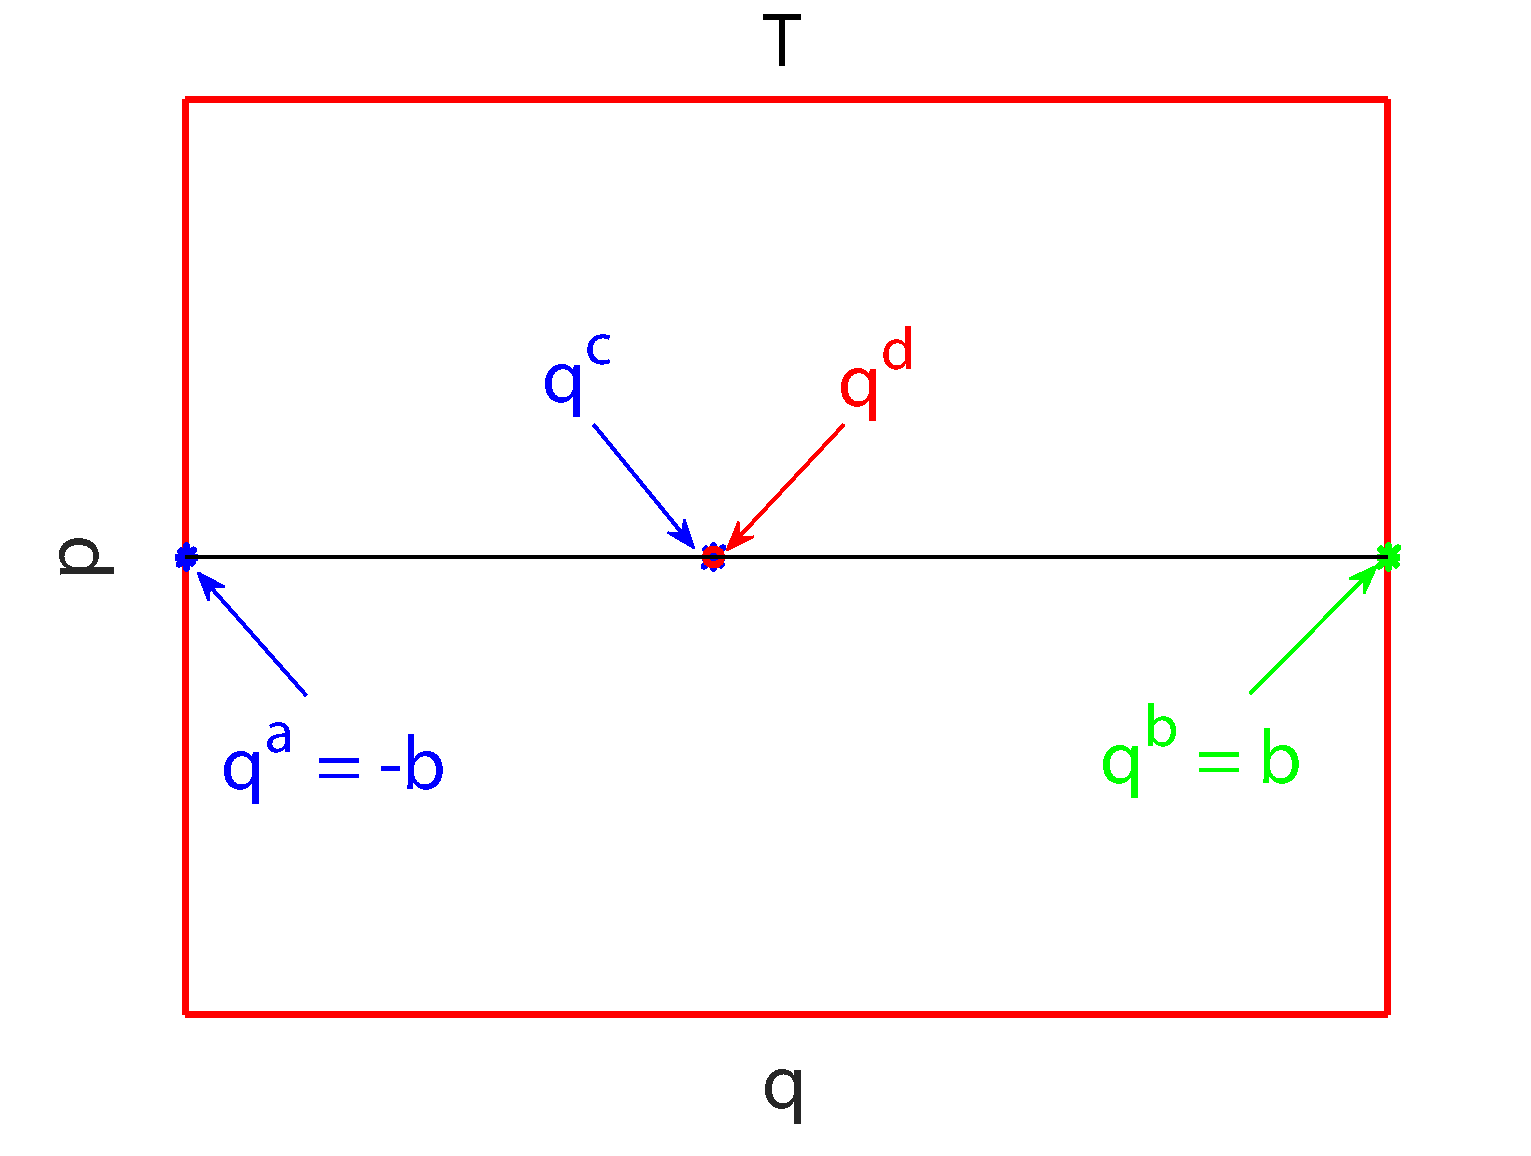
\includegraphics[width=0.7\textwidth]{T4_1_example}
  \end{center}
  \caption{\textbf{Bisection in target PS \set{T}{}{}.} Algorithm \ref{alg:bisection} is run for the interval $[\variabile{q}^{\textrm{a}}, \variabile{q}^{\textrm{b}}]$ along direction $\variabile{p}=0$. The coordinates $\variabile{q}^{\textrm{c}}$ and $\variabile{q}^{\textrm{d}}$ are found such that 
$|\variabile{q}^{\textrm{c}}-\variabile{q}^{\textrm{d}}|<\textrm{tol}$. $\Pi^{\textrm{c}}= \Pi^{\textrm{a}}$ and $\Pi^{\textrm{d}}\neq \Pi^{\textrm{a}}$.}
\label{fig:bisec}
 \end{figure}
\\ \indent Now, if $\lineaj\neq1$ the procedure applied to the interval 
$[\variabile{q}^{\textrm{a}}(\variabile{p}), \variabile{q}^{\textrm{b}}(\variabile{p})]$ needs to be applied to $[\variabile{q}^{\textrm{a}}(\variabile{p}),\variabile{q}^{\textrm{c}}(\variabile{p})]$ until the source is reached, i.e., until $\lineaj=1$. If $\lineaj=1$, the source is reached by the rays traced back from the target. This means that a possible path $\Pi^{\textrm{a}}$ from \point{S} to \point{T} is found and the position coordinates $\variabile{q}^{\textrm{\,min}}(\Pi^{\textrm{a}}, \variabile{p})$ and $\variabile{q}^{\textrm{\,max}}(\Pi^{\textrm{a}}, \variabile{p})$ are determined and the intensity is updated according to (\ref{eq:intensity_brm}).
%Next, all the possible paths along direction $\variabile{p}$ are detected by sequentially applying bisection until all the interval $[\variabile{q}^{\textrm{a}}(\variabile{p}), \variabile{q}^{\textrm{b}}(\variabile{p})]$ is investigated. 
\\ \indent 
Finally, to detect all possible paths that can occur along direction $\variabile{p}$ the procedure explained above is applied also to the interval $[\variabile{q}^{\textrm{d}}(\variabile{p}), \variabile{q}^{\textrm{b}}(\variabile{p})]$ along direction $\variabile{p}$ continuing until the entire interval $[\variabile{q}^{\textrm{a}}(\variabile{p}), \variabile{q}^{\textrm{b}}(\variabile{p})]$ is investigated. 
The main steps of the method are outlined in the following.
\begin{enumerate}
\item Given a direction \variabile{p}, the end points $(\variabile{q}^{\,\textrm{a}}, \variabile{p})$ and $(\variabile{q}^{\,\textrm{b}}, \variabile{p})$ of the target PS \set{T}{}{}, where $\variabile{q}^{\,\textrm{a}} = -\variabile{b}$, $\variabile{q}^{\,\textrm{b}} = \variabile{b}$. Start from $\lineai=\nline$.
\item \label{ray trace} Using backward ray tracing, trace back from line $\lineai$ the rays with parametrizations $\vect{r}_{\textrm{a}}(s)$ and $\vect{r}_\textrm{b}(s)$ corresponding to the position coordinates $(\variabile{x}_{\lineai}^{\,\textrm{a}}, \variabile{z}_{\lineai}^{\,\textrm{a}})$ and $ (\variabile{x}_{\lineai}^{\,\textrm{b}}, \variabile{z}_{\lineai}^{\,\textrm{b}})$ and the angular coordinates $\optangle_{\lineai}^{\textrm{a}}$ and $\optangle_{\lineai}^{\textrm{b}}$, respectively. 
%considering the directions $\variabile{p}_{\lineai}^{\,\textrm{a}}$ and $\variabile{p}_{\lineai}^{\,\textrm{b}}$ with respect to the optical axis. 
%We remind the reader that we indicate with $\variabile{p}_{\lineai}^{\,\textrm{a}}$ and $\variabile{p}_{\lineai}^{\,\textrm{b}}$ on \set{T}{\lineai}{} the rays directions with respect to the normal of line $\lineai$. Hence, if $\lineai=\nline $ then $\variable{p}_{\lineai}^{\,\textrm{a}}=\variabile{p}_{\lineai}^{\,\textrm{b}}=\variabile{p}$, otherwise $\variabile{p}_{\lineai}^{\,\textrm{a}}\neq\variabile{p}_{\lineai}^{\,\textrm{b}}$.
\item Determine indices $\lineaj\neq\lineai$ and $\lineak\neq\lineai$ of the lines from which the rays with parametrizations $\vect{r}_{\textrm{a}}(s)$ and $\vect{r}_{\textrm{b}}(s)$ originated.
\item Consider the new rays parametrization $\vect{r}_{\textrm{a}}(s)$ and $\vect{r}_{\textrm{b}}(s)$ corresponding to the coordinates $(\variabile{x}_{\lineaj}^{\textrm{a}}, \variabile{z}_{\lineaj}^{\textrm{a}})$, $\optangle_{\lineaj}^{\textrm{a}}$ and $(\variabile{x}_{\lineak}^{\textrm{a}}, \variabile{z}_{\lineak}^{\textrm{b}})$, $\optangle_{\lineak}^{\textrm{b}}$, respectively.
\item Update the paths $\Pi^\textrm{a}$ and $\Pi^\textrm{b}$: $\Pi^\textrm{a} = (\lineaj, \Pi^{\textrm{a}})$ and $\Pi^\textrm{b} = (\lineak, \Pi^\textrm{b})$
\item If $\lineaj=\lineak \neq 1$ and $\lineaj=\lineak \neq \nline$
\begin{itemize}
\item Set $\lineai=\lineaj$
%\item Consider the coordinates of rays $\vect{r}_{\textrm{a}}$ and $\vect{r}_{\textrm{b}}$ on line $\lineaj$ 
\item Restart the procedure from point $\ref{ray trace}$
\end{itemize}
\item If $\lineaj=\lineak= 1$ 
\begin{itemize}
\item A relevant path $\Pi^{\textrm{a}} = \Pi^{\textrm{b}}$ is found. 
\item Determine 
\begin{equation*}
\begin{aligned}
\variabile{q}^{\textrm{min}}(\Pi^{\textrm{a}}, \variabile{p})&=\min\{\variabile{q}^{\textrm{a}}(\Pi^{\textrm{a}}, \variabile{p}), \variabile{q}^{\textrm{b}}(\Pi^{\textrm{b}}, \variabile{p})\}\\ 
\variabile{q}^{\textrm{max}}(\Pi^{\textrm{a}}, \variabile{p})&=\max\{\variabile{q}^{\textrm{a}}(\Pi^{\textrm{a}}, \variabile{p}), \variabile{q}^{\textrm{b}}(\Pi^{\textrm{b}}, \variabile{p})\}.
\end{aligned}
\end{equation*}
\item Update the intensity $$I(\variabile{p}) = I(p)+\variabile{q}^{\textrm{max}}(\Pi^{\textrm{a}}, \variabile{p})-\variabile{q}^{\textrm{min}}(\Pi^{\textrm{a}}, \variabile{p})$$
\end{itemize}
%\item If $\lineaj=\lineak= \nline$ stop the procedure (the rays reach the target again).
\item If $\lineaj\neq\lineak$ 
\begin{itemize}
\item Apply the bisection method to the interval $[\variabile{q}^{\textrm{a}}, \variabile{q}^{\textrm{b}}]$ along direction $\variabile{p}$, given the points $(\variabile{q}^{\,\textrm{c}}, \variabile{p})$ and $(\variabile{q}^{\,\textrm{d}}, \variabile{p})$ in target PS \set{T}{}{} such that $|\variabile{q}^{\,\textrm{c}}-\variabile{q}^{\,\textrm{d}}|<\textrm{tol}$. 
\item If $\lineaj\neq\nline$
\begin{itemize}
\item Set $\variabile{q}^{\textrm{b}} = \variabile{q}^{\textrm{c}}$,
\item Set $(\variabile{x}_{\lineaj}^{\textrm{b}}, \variabile{z}_{\lineaj}^{\textrm{b}}) = (\variabile{x}_{\lineaj}^{\textrm{c}}, \variabile{z}_{\lineaj}^{\textrm{b}})$ and $\optangle_{\lineaj}^{\textrm{b}}= \optangle_{\lineaj}^{\textrm{c}}$
\item Set $\lineai = \lineaj$
\item Restart from $\ref{ray trace}$ with the updated coordinates,
\end{itemize}
\item Update $\variabile{q}^{\textrm{a}}= \variabile{q}^{\textrm{d}}$,
\item $\Pi^{\textrm{a}} = \Pi^{\textrm{c}}$
\item Update $(\variabile{x}_{\lineaj}^{\textrm{a}}, \variabile{z}_{\lineaj}^{\textrm{a}}) = (\variabile{x}_{\lineaj}^{\textrm{d}}, \variabile{z}_{\lineaj}^{\textrm{d}})$ and $\optangle_{\lineaj}^{\textrm{a}}= \optangle_{\lineaj}^{\textrm{d}}$
\item Restart from $\ref{ray trace}$
\end{itemize}
\end{enumerate}
Giving as input $I(\variabile{p})=0$ for every direction $\variabile{p}$ and the tolerance $\textrm{tol}=10^{-12}$,
the method is defined in the recursive Algorithm \ref{alg:recursiveraymapping}.
\begin{algorithm}
\caption{Recursive function for direct backward ray mapping}\label{alg:recursiveraymapping}
Initialize: $\lineai = \nline$, $\variabile{q}^{\,\textrm{a}}= \variabile{x}^{\,\textrm{a}}_{\lineai}=-\variabile{b}$, $\variabile{q}^{\,\textrm{b}}= \variabile{x}^{\,\textrm{b}}_{\lineai}=\variabile{b}$, $\dir{}{}=\optangle^{\textrm{a}}_\lineai=\optangle^{\textrm{b}}_\lineai=\textrm{const}$, $\variabile{z}_{\lineai}^{\textrm{a}}=\variabile{z}_{\lineai}^{\textrm{b}}= \variabile{h}$, $\Pi^{\textrm{a}}=({\nline})$.
\begin{algorithmic}[1]
\Procedure{Intensity computation}{$\variabile{q}^{\,\textrm{a}}$,  $\variabile{q}^{\,\textrm{b}}$, $\variabile{x}^{\,\textrm{a}}_{\lineai},$  $\variabile{x}^{\,\textrm{b}}_{\lineai},$ $\variabile{z}^{\,\textrm{a}}_{\lineai},$  $\variabile{z}^{\,\textrm{b}}_{\lineai},$ $\dir{}{}$, $\optangle^{\textrm{a}}_{\lineai}$, $\optangle^{\textrm{b}}_{\lineai}$, $\Pi^{\textrm{a}}$, $\lineai$}
\State Apply backward ray tracing to $(\variabile{x}^{\,\textrm{a}}_{\lineai},\variabile{z}^{\textrm{a}}_{\lineai})$, $\optangle_{\lineai}^{\textrm{a}}$ and $(\variabile{x}^{\,\textrm{b}}_{\lineai},\variabile{z}^{\textrm{b}}_{\lineai})$, $\optangle_{\lineai}^{\textrm{b}}$ \State Determine the lines $\lineaj\neq\lineai$ and $\lineak\neq\lineai$ from which $\vect{r}_{\textrm{a}}(s)$ and $\vect{r}_{\textrm{b}}(s)$ are emitted.
\State Update path $\Pi^{\textrm{a}}=(\lineaj, \Pi^{\textrm{a}})$
\State Calculate the position coordinates $(\variabile{x}^{\,\textrm{a}}_{\lineaj},\variabile{z}^{\textrm{a}}_{\lineaj})$, $(\variabile{z}^{\,\textrm{b}}_{\lineaj}, \variabile{p}^{\textrm{b}}_{\lineaj})$ and $\optangle_{\lineaj}^{\textrm{a}}$, $\optangle_{\lineaj}^{\textrm{b}}$.
\If {$\lineaj = \lineak$}
\If{$\lineaj\neq1$}
\State\Return{\Call{Intensity computation}{$\variabile{q}^{\,\textrm{a}},$  $\variabile{q}^{\,\textrm{b}},$ $\variabile{x}^{\,\textrm{a}}_{\lineaj},$ $\variabile{x}^{\,\textrm{b}}_{\lineaj},$ $\variabile{z}^{\,\textrm{a}}_{\lineaj},$ $\variabile{z}^{\,\textrm{b}}_{\lineaj},$ $\dir{}{}$, $\optangle^{\textrm{a}}_{\lineaj}$, $\optangle^{\textrm{b}}_{\lineaj}$, $\Pi^{\textrm{a}}$, $\lineaj$}}
\Else  \State Calculate
$\variabile{q}^{\textrm{min}} = \min\{\variabile{q}^{\textrm{a}}, \variabile{q}^{\textrm{b}}\}$, $\variabile{q}^{\textrm{max}} = \max\{\variabile{q}^{\textrm{a}}, \variabile{q}^{\textrm{b}}\}$
\State Assume Lambertian source
\State $I(\dir{}{}) = I(\dir{}{})+\variabile{q}^{\textrm{max}}(\Pi^{\textrm{a}}, \dir{}{})
-\variabile{q}^{\textrm{min}}(\Pi^{\textrm{a}}, \dir{}{})$ 
\EndIf
\Else 
\State Apply bisection to the segment $[\variabile{q}^{\,\textrm{a}}(\Pi^\textrm{a}, \dir{}{}), \variabile{q}^{\,\textrm{b}}(\Pi^\textrm{b}, \dir{}{})]$
\State Find the target coordinates $(\variabile{q}^{\,\textrm{c}},\variabile{p})$ and $(\variabile{q}^{\,\textrm{d}},\variabile{p})$ of the rays with parame\-trization $\vect{r}_{\textrm{c}}$ and $\vect{r}_{\textrm{d}}$, such that $$|\variabile{q}^{\,\textrm{c}}-\variabile{q}^{\,\textrm{d}}|<\textrm{tol}$$
\If {$\lineaj\neq \nline$}
\State\Return{\Call{Intensity computation}{$\variabile{q}^{\,\textrm{a}},$  $\variabile{q}^{\,\textrm{c}},$ $\variabile{x}^{\,\textrm{a}}_{\lineaj},$ $\variabile{x}^{\,\textrm{c}}_{\lineaj},$ $\variabile{z}^{\,\textrm{a}}_{\lineaj},$ $\variabile{z}^{\,\textrm{c}}_{\lineaj},$ $\dir{}{}$, $\optangle^{\textrm{a}}_{\lineaj}$, $\optangle^{\textrm{c}}_{\lineaj}$, $\Pi^{\textrm{a}}$,~$\lineaj$}}
\EndIf 
\State\Return{\Call{Intensity computation}{$\variabile{q}^{\,\textrm{d}},$  $\variabile{q}^{\,\textrm{b}},$ $\variabile{x}^{\,\textrm{d}}_{\lineaj},$ $\variabile{x}^{\,\textrm{b}}_{\lineaj},$ $\variabile{z}^{\,\textrm{d}}_{\lineaj},$ $\variabile{z}^{\,\textrm{b}}_{\lineaj},$ $\dir{}{}$, $\optangle^{\textrm{d}}_{\lineaj}$, $\optangle^{\textrm{b}}_{\lineaj}$, $\Pi^{\textrm{d}}$, $\lineaj$}}
\EndIf
\EndProcedure
\end{algorithmic}
\end{algorithm}
\\ \indent The procedure is able to determine all the possible paths that the rays can follow during their propagation from \set{S}{}{} to \set{T}{}{}. Also, rays located on the boundaries of the regions with positive luminance in target PS \set{T}{}{} are found.
The method is summarized by the flowchart in Figure \ref{fig:flowchart_raymapping}
\begin{figure}[t]
  \begin{center}
  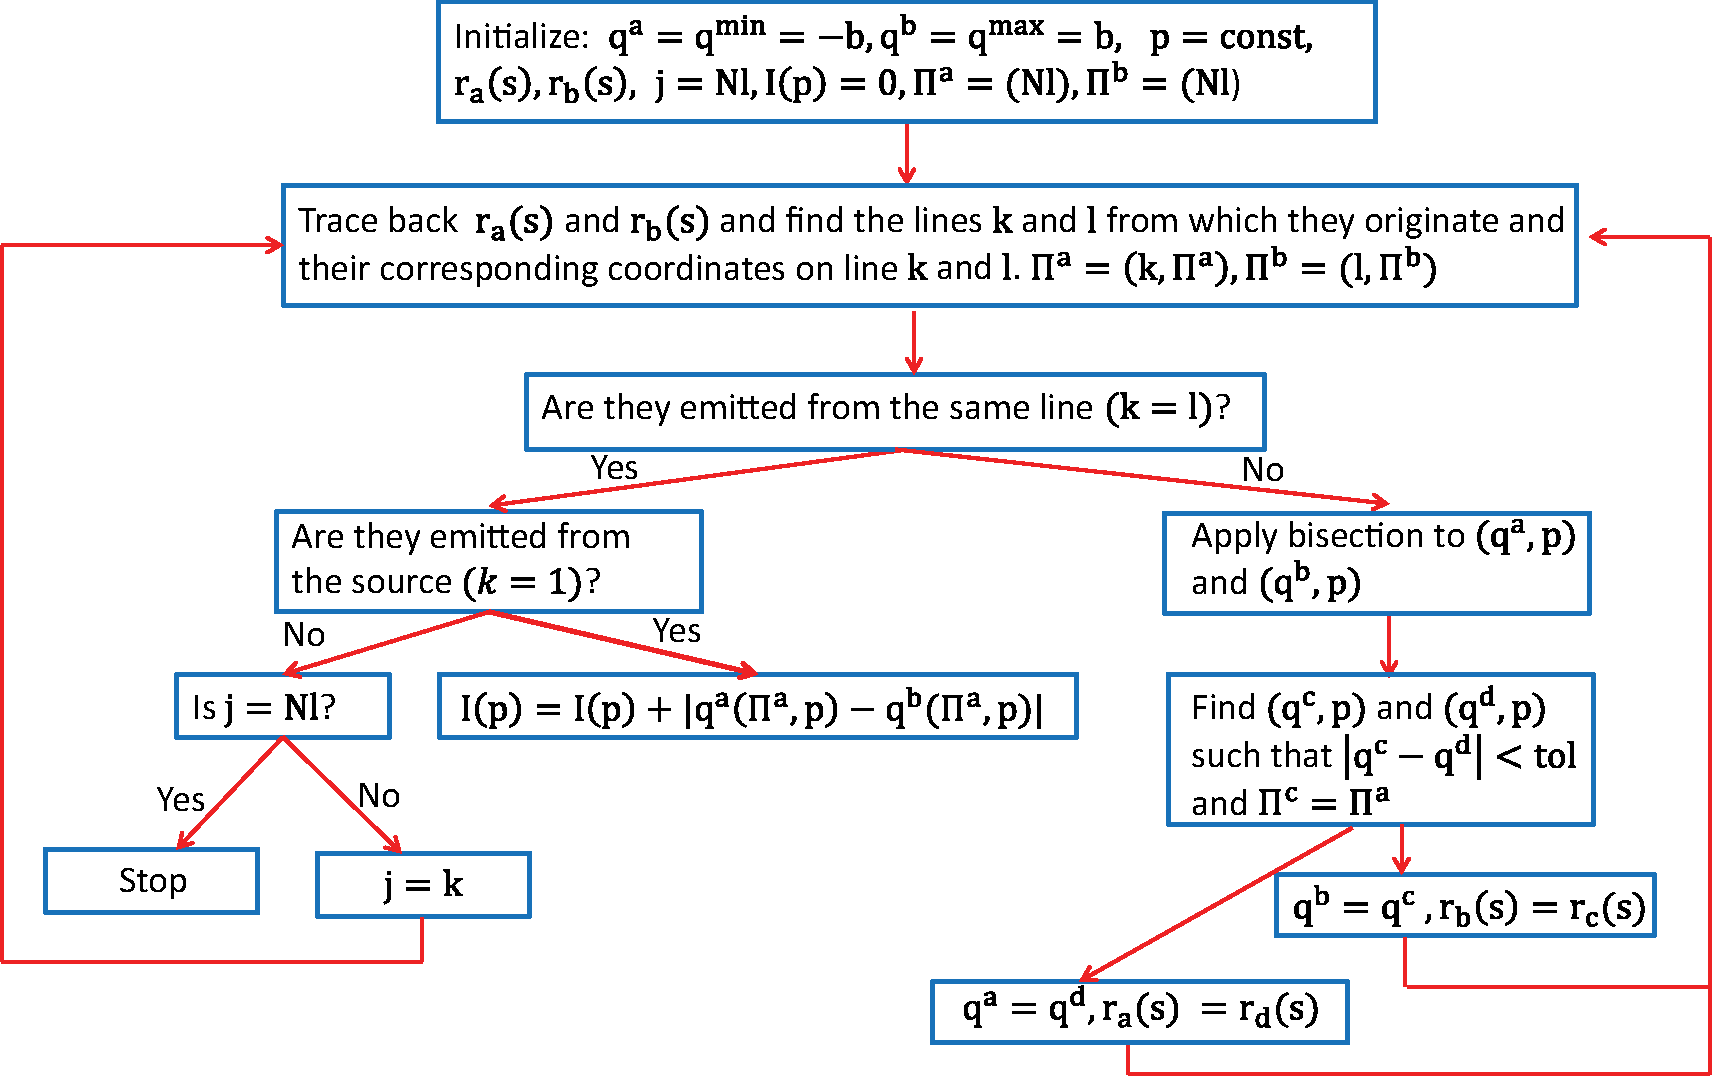
\includegraphics[width=\textwidth]{flowchart_raymapping}
  \end{center}
  \caption{\textbf{Main steps of direct backward ray mapping modified for systems with curved lines.}}
\label{fig:flowchart_raymapping}
 \end{figure}
\\ \indent
Next, the method is applied to two optical systems formed by curved lines. In the next section we show the results for the TIR-collimator and in Section \ref{sec:PR} we provide numerical results for the parabolic reflector.
\section{Results for the TIR-collimator}\label{sec:TIR}
% Introduction 
In this section we apply modified backward ray mapping to the TIR-collimator presented in Chapter \ref{chap:boundaries_alpha} and depicted in Figure \ref{fig:analyticlens}. The target PS of this system is the rectangular \set{T}{}{}$= [-\variabile{b}, \variabile{b}]\times[-1,1]$ with $\variabile{b}=9.7$. The aim is to detect all the possible path $\Pi$ and the rays located on the boundaries $\partial$\set{R}{}{}$(\Pi)$ of the corresponding regions in target PS. 
\\ \indent In Chapter \ref{chap:boundaries_alpha}, we found five different paths for the TIR-collimator (see Figure \ref{fig:Tir2}). The boundaries of the corresponding regions in target PS \set{T}{}{} are in general difficult to approximate. Furthermore, along one direction $\dir{}{}$ more than two points can be located on the boundary $\partial$\set{R}{}{}$(\Pi)$ \set{R}{}{}$(\Pi)$ corresponding to a certain path $\Pi$. To determine properly all the boundaries 
$\partial$\set{R}{}{}$(\Pi)$, we need to divide the interval $[-\variabile{b}, \variabile{b}]$ in 
\set{T}{}{} into intervals of the same length. Hence, we consider a partitioning 
$Q = -\variabile{b}=\variabile{q}^{0}<\variabile{q}^{1}<\cdots<\variabile{q}^{\textrm{Ni}}=\variabile{b}$ of $[-\variabile{b}, \variabile{b}]$ where $\textrm{Ni}$ is the total number of sub-intervals along the $\variabile{q}$-axis.
For each direction $\dir{}{}\in [-1,1]$ the procedure explained in Section \ref{sec:raymapping_explanation} is repeated for every sub-interval $[\variabile{q}^{\textrm{k}}(\dir{}{}), \variabile{q}^{\textrm{k}+1}(\dir{}{})]\subset [\variabile{q}^{\textrm{a}}(\dir{}{}), \variabile{q}^{\textrm{b}}(\dir{}{})]$ with $\textrm{k}=0, \cdots, \textrm{Ni}-1$ and $\variabile{q}^{\textrm{a}}(\dir{}{}) = -\variabile{b}$ and $\variabile{q}^{\textrm{b}}(\dir{}{}) = \variabile{b}$.\\ \indent
To establish in how many sub-intervals \textrm{Ni} we need to divide the target, we exploit \'{e}tendue conservation. We use the same idea applied to determine the value of $\alpha$ for the $\alpha$-shapes method and to provide a stopping criterion for the triangulation refinement (see Chapters \ref{chap:boundaries_alpha} and \ref{chap:triangulation}). 
The source \'{e}tendue $U_1$ is calculated from (\ref{eq:Usource}), obtaining $U_1 \approx 7.7$. The target \'{e}tendue $U_\textrm{t}$ is given by Equation (\ref{eq:etenduetarg1}). $U_\textrm{t}$ is calculated several times considering every time a different partitioning $Q$ for the $\variabile{q}$-axis of the target PS. Next, the absolute value of the difference between the source and target \'{e}tendue is obtained from
\begin{equation}\label{eq:delta_raymapping}
\Delta U =  \big|U_1-U_{\textrm{t}}\big|.
\end{equation}
If a small value of $\Delta U$ is obtained, then a good approximation of $U_{\textrm{t}}$ is found and therefore, the partition $Q$ used for the computation of $U_{\textrm{t}}$ is suitable for detecting correctly the boundaries $\partial$\set{R}{}{}$(\Pi)$. In Figure \ref{fig:etendue_raymapping_tir} we show how $\Delta U$ decreases by increasing the number of sub-intervals $\textrm{Ni}$ in the partitioning $Q$.  
\begin{figure}[h]
  \begin{center}
  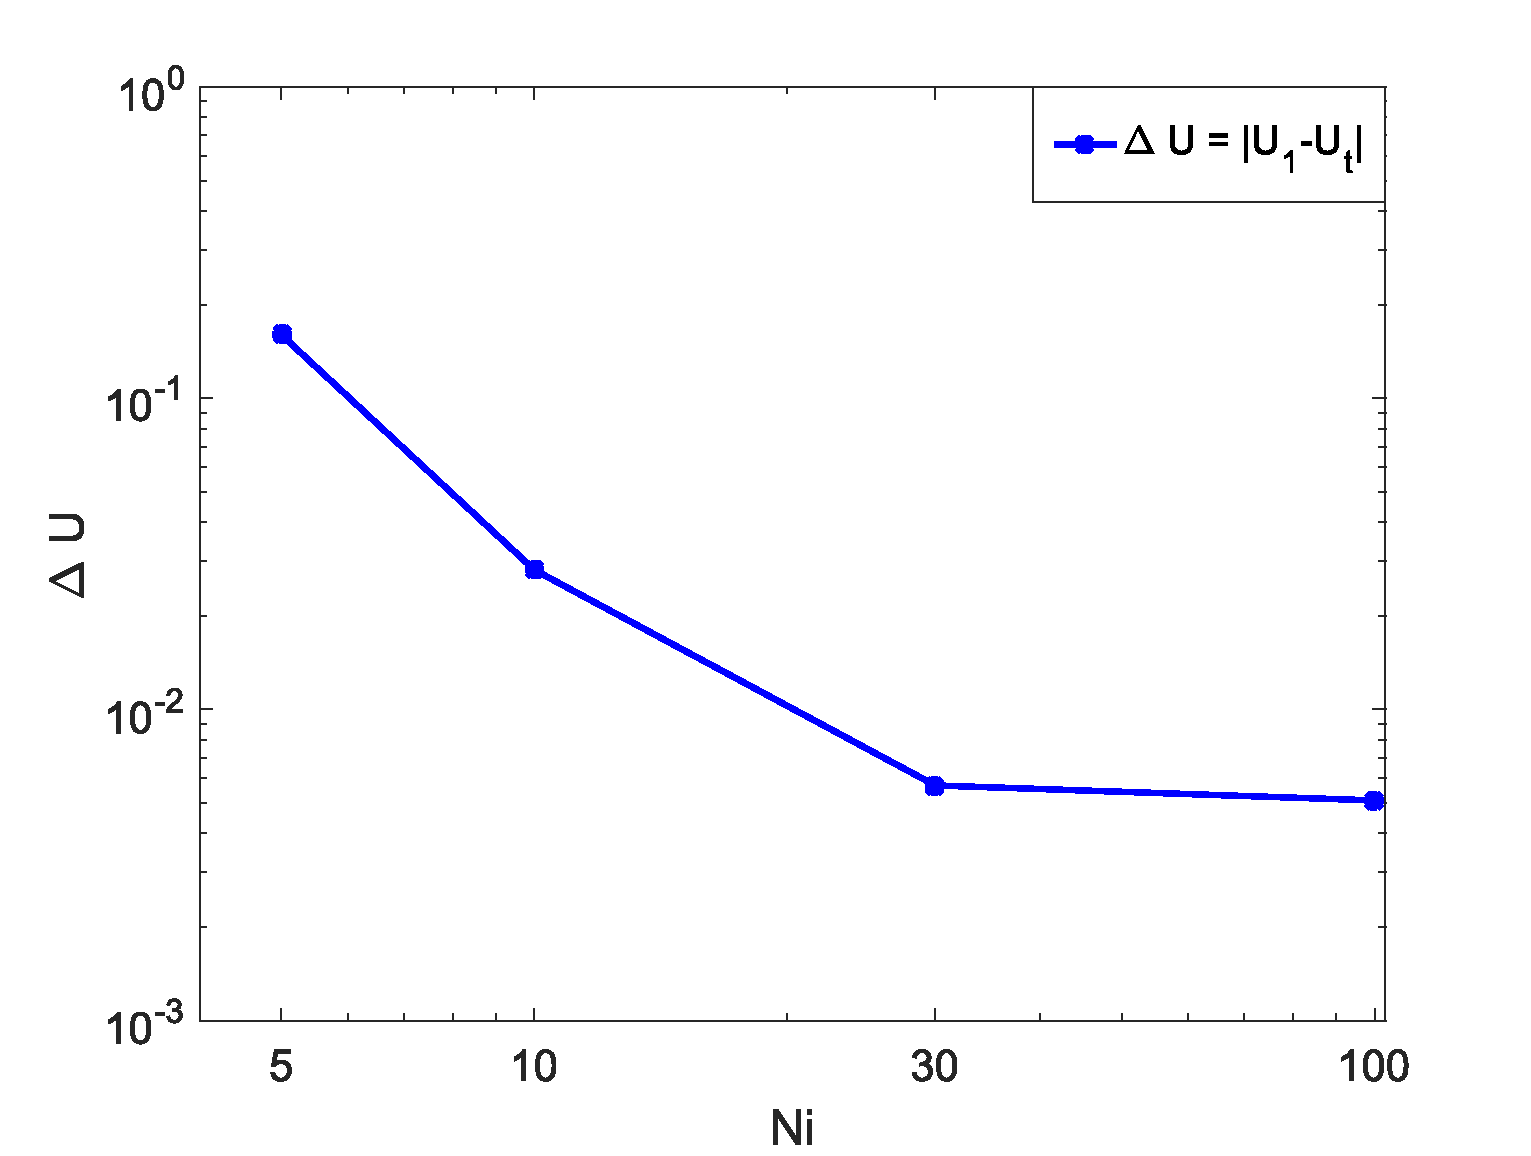
\includegraphics[width=0.7\textwidth]{etendue_raymapping_tir}
  \end{center}
  \caption{\textbf{Difference between the source and the target \'{e}tendue for the TIR-collimator.} $U_{\textrm{t}}$ is computed four times increasing every time the number of bins $\textrm{Ni}$ where $\textrm{Ni}\in\{5,10,30,100\}$. }
\label{fig:etendue_raymapping_tir}
 \end{figure}
In Figure \ref{fig:boundaries_TIR_ray_mapping} we show the distribution of the rays traced using the backward ray mapping method with $\textrm{Ni}=30$ and $\nbin = 100.$ 
\begin{figure}[h]
  \begin{center}
  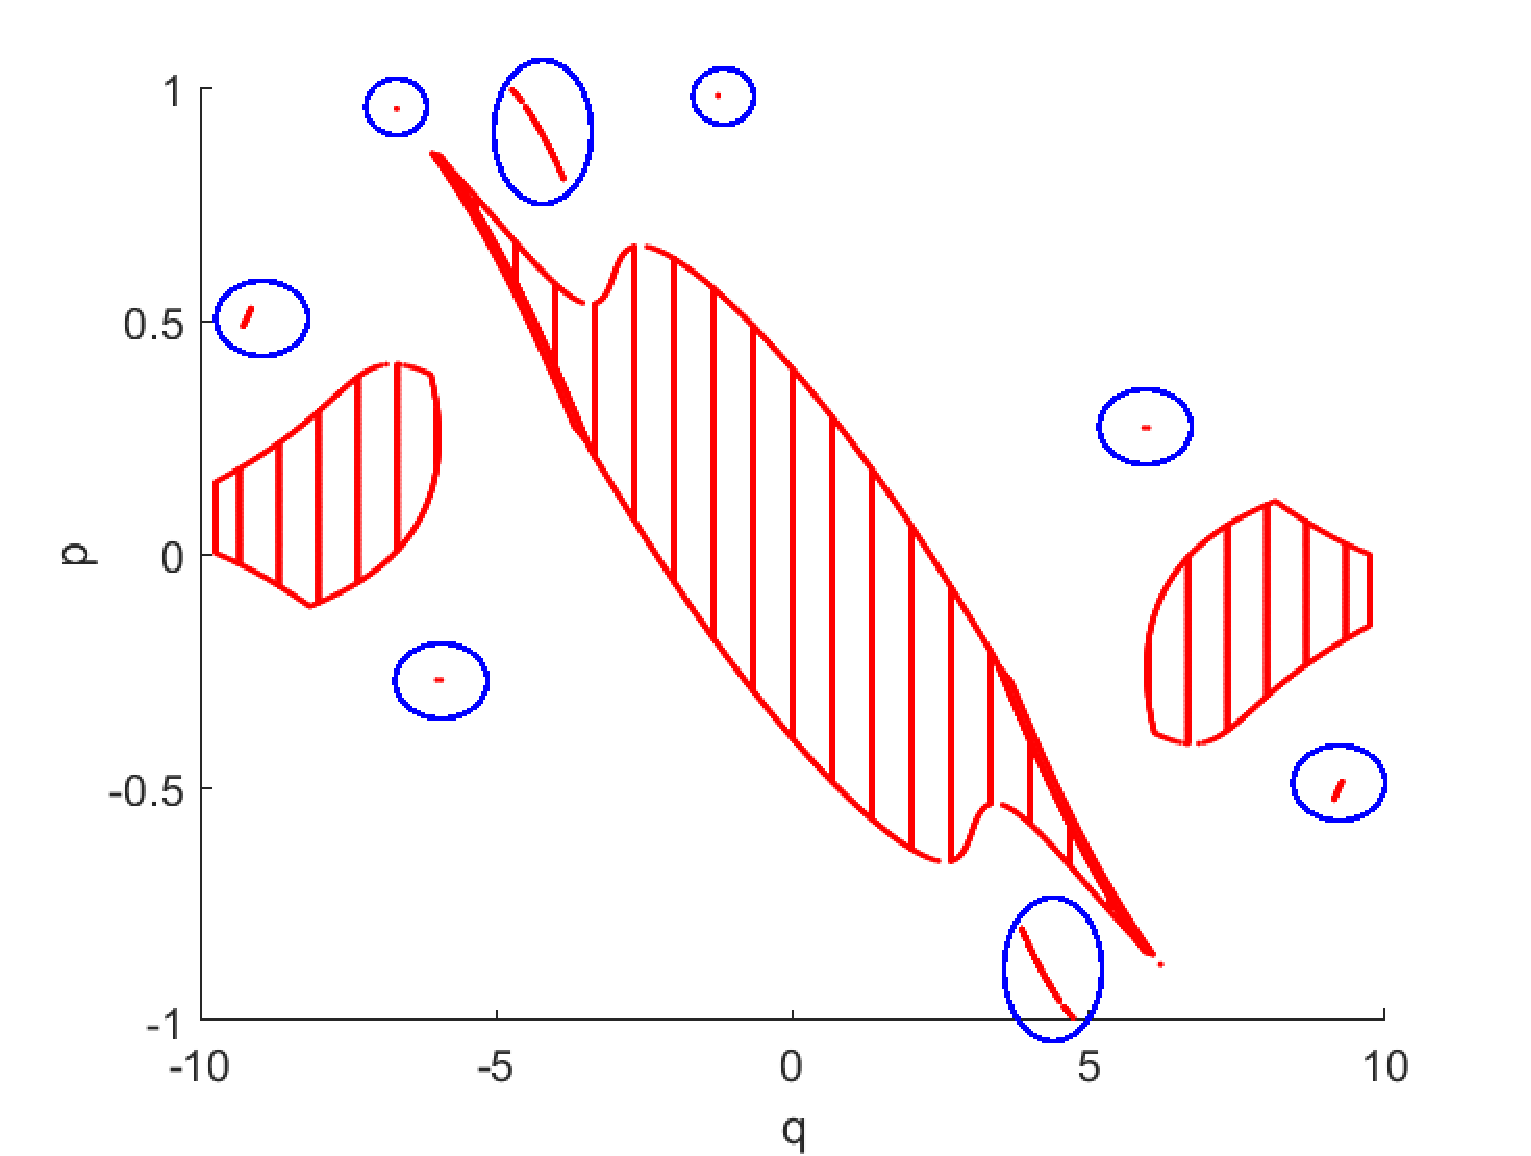
\includegraphics[width=0.7\textwidth]{boundaries_ray_mapping_tir}
  \end{center}
  \caption{\textbf{Ray distribution at target PS of the TIR-collimator.}
 The $\variabile{q}$-axis is divided into $\textrm{Ni}=30$ bins, the $\variabile{p}$-axis is divided into $\nbin = 100$ bins. Approximately $6*10^3$ rays are traced from the target to the source (red dots). Because of numerical errors, a few rays outside the region with positive luminance are found (rays rimmed in blue).}
\label{fig:boundaries_TIR_ray_mapping}
 \end{figure}
In this case, backward ray mapping detects $11$ different paths from the source to the target. 
We observe that only $5$ of them are the paths that we expect from PS ray tracing, which are:
\begin{equation}\label{eq:paths_tir}
\begin{array}{llll}
\Pi_1&=(1,2,7,12), \\
\Pi_2&=(1,4,6,7,12), & \Pi_3&=(1,10,8,7,12),\\
\Pi_4&=(1,3,7,12), & \Pi_5&=(1,11,7,12).
\end{array}\end{equation}
%(see Chapter \ref{chap:boundaries_alpha}). 
Backward ray mapping also detect the spurious paths:
\begin{equation}\label{eq:paths_tir}
\begin{array}{llll}
\Pi_6&=(1,2,9,8,7,12), & \Pi_7&=(1,2,5,6,7,12), \\
\Pi_8&=(1,2,2,7,12),& \Pi_9&=(1,7,12),\\
\Pi_{10}&=(1,2,4,6,7,12),& \Pi_{11}&=(1,2,10,8,7,12).
\end{array}\end{equation}
These paths are due to numerical errors, the corresponding rays are rimmed in blue in Figure \ref{fig:boundaries_TIR_ray_mapping}. Note that some rays inside different circles might correspond to the same path. The numerical error can be related to the precision of the bisection method and the numerical computation of the intersection points when backward ray tracing is used. We remark that in backward ray tracing, the intersection between the ray and the lens (line $2$) is computed using the Newton-Raphson procedure.
To detect only the boundaries of the regions formed by the rays that follow a \textit{real} path $\Pi_{\variabile{j}}$, with $\variabile{j}\in\{1, \cdots, 5\}$, we check the index of refraction that every ray has once it arrives at the source.
If this is equal to the same index of \point{S} ($\n=1$ for the TIR-collimator), then the ray follows a physical path, otherwise it follows one of the paths in (\ref{eq:paths_tir}) and, therefore, it is not considered for the intensity calculation. This gives the ray distribution at the target PS shown in Figure \ref{fig:boundaries_TIR_ray_mapping1}. We observe that, discarding those rays, $5$ different paths are found. These are the same paths we obtained using PS ray tracing.
\begin{figure}[h]
  \begin{center}
  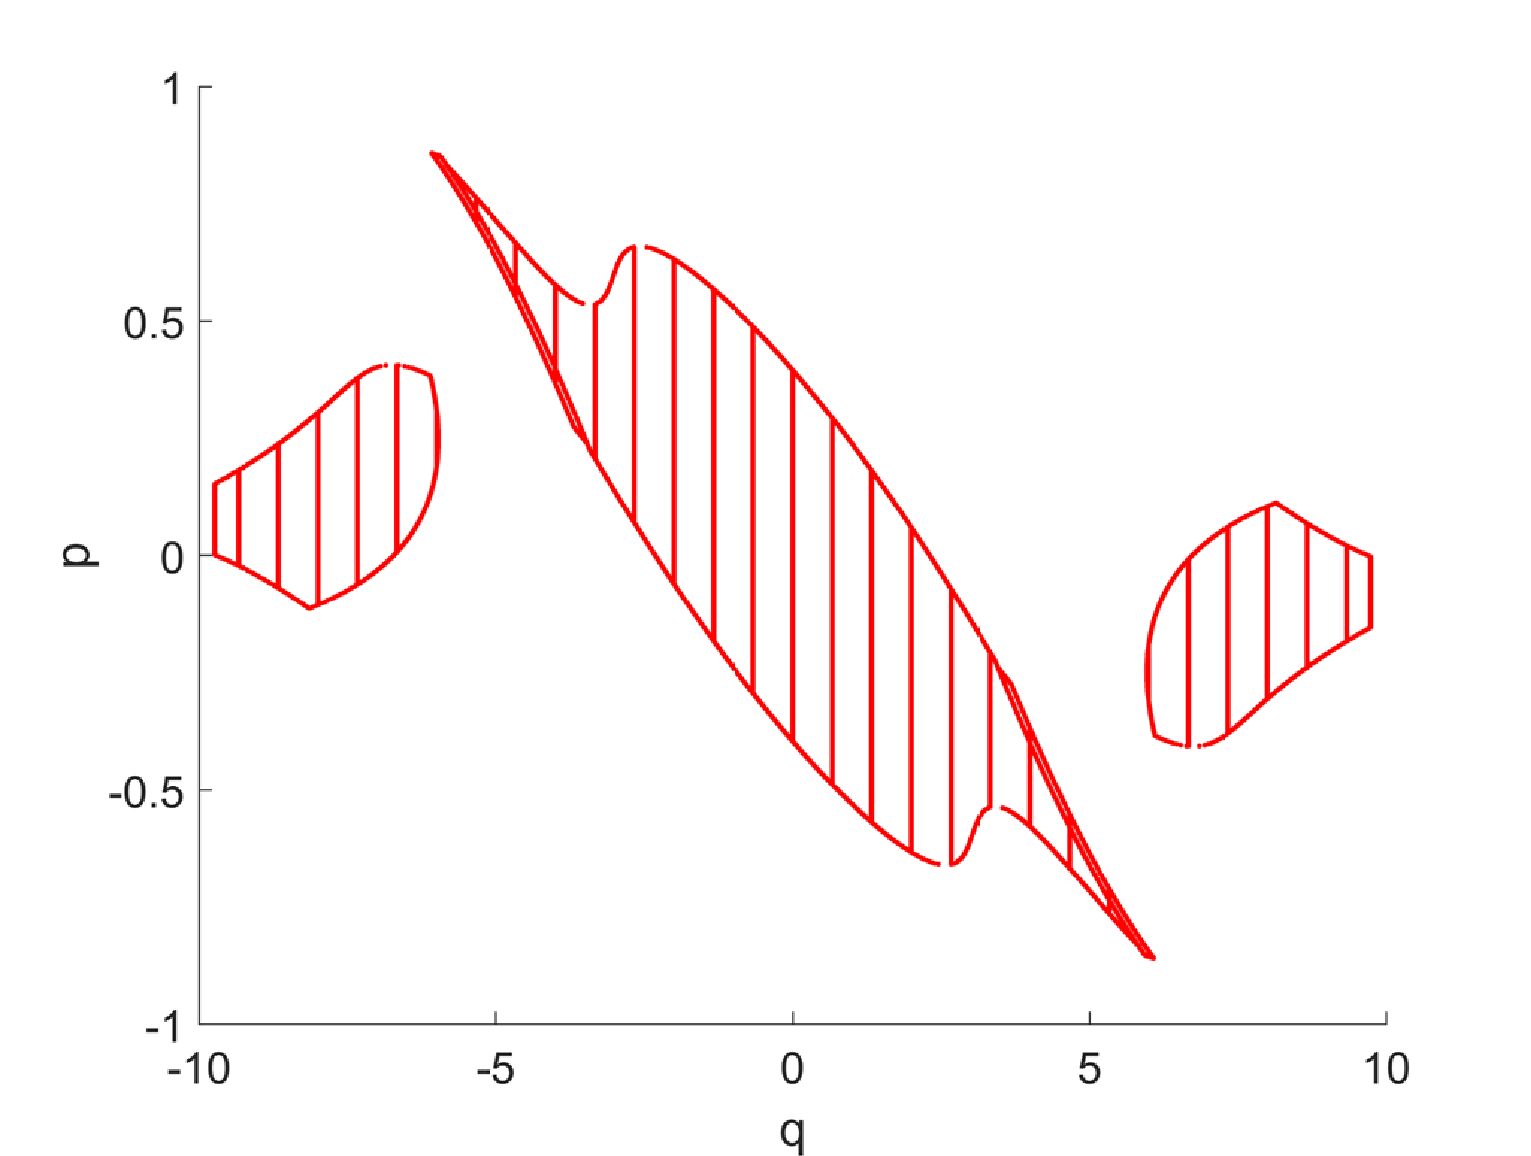
\includegraphics[width=0.7\textwidth]{boundaries_ray_mapping_tir2}
  \end{center}
  \caption{\textbf{Ray distribution at target PS of the TIR-collimator.}
 The $\variabile{q}$-axis is divided into $\textrm{Ni}=30$ bins, the $\variabile{p}$-axis is divided into $\nbin = 100$ bins. Considering only the rays that arrive to the source with the correct index of refraction ($\n=1$), the regions with positive luminance are computed correctly.}
\label{fig:boundaries_TIR_ray_mapping1}
 \end{figure}
Figure \ref{fig:boundaries_TIR_ray_mapping1} shows that the rays on the boundaries $\partial$\set{R}{}{}$(\Pi_{\variabile{j}})$ are determined for every path $\Pi_{\variabile{j}}$ with $\variabile{j}\in\{1, \cdots, 5\}$. The ability of the backward ray mapping method to recognize spurious paths makes it suitable to detect ghost stray light, which is unwanted light that reduce the performance of optical systems \cite{breault1995control}. Optical designers are interested in developing methods for minimizing stray light intensity \cite{grabarnik2015optical}. Backward ray mapping could be an alternative approach for such purpose. 
\\ \indent Note that some rays in the interior of the regions are still traced because we divided the target PS along the $\variabile{q}$-axis into $\textrm{Ni}=30$ bins. As a consequence, also the rays located at the end points of every bin are traced. \\
\indent The target ray mapping intensity $\hat{I}_{\textrm{RM}}$ is calculated using Equation (\ref{eq:Ips}). The profile of $\hat{I}_{\textrm{RM}}$ with $\textrm{Ni}=30$ is depicted in Figure \ref{fig:intensity_tir_raymapping} with the red line. It is compared with the reference intensity (blue line) which is given by QMC ray tracing with $10^7$ rays. The picture shows that the backward ray mapping method calculates the intensity correctly.
\begin{figure}[t]
  \begin{center}
  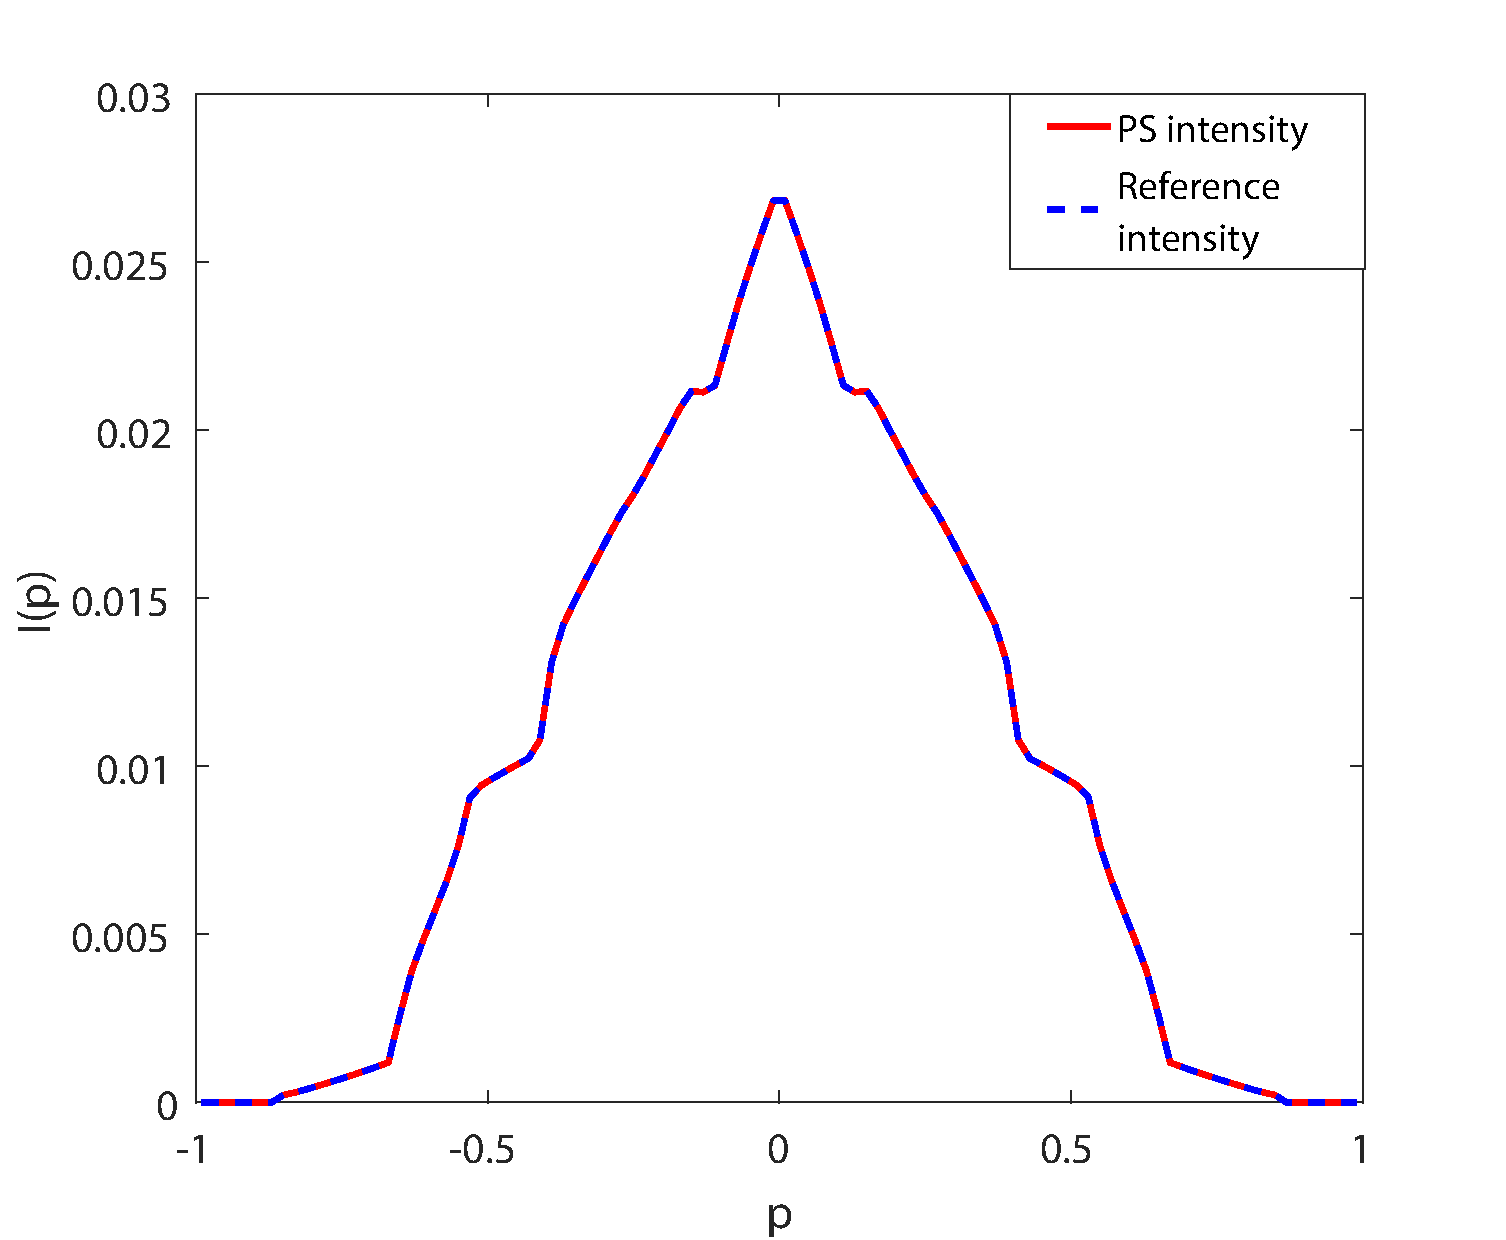
\includegraphics[width=0.7\textwidth]{intensity_tir_raymapping}
  \end{center}
  \caption{\textbf{Profile of the intensity for the TIR-collimator.}
 The ray mapping intensity is calculated dividing the $\variabile{q}$-axis into $\textrm{Ni}=30$ bins. The reference intensity is obtained from QMC ray tracing with $10^7$ rays.}
\label{fig:intensity_tir_raymapping}
 \end{figure}
\\ \indent 
Finally, we compare backward ray mapping with QMC ray tracing. The errors are obtained from (\ref{eq:error}) and are shown in a logarithmic scale in Figure \ref{fig:error_tir_raymapping} as a function of the CPU-time. The approximation of the RM intensity $\hat{I}_{\textrm{RM}}$ is improved by increasing the number of bins $\textrm{Ni}$ in the partitioning $Q$. The approximated QMC intensity $\hat{I}_{\textrm{QMC}}$ is calculated several times gradually increasing the number of rays $\nrays$. Both intensities are computed using the same number of bins, $\nbin=100$ in the partitioning $P$ of the $\variabile{p}$-axis. The minimum ray mapping error is obtained with $\textrm{Ni}=100$ bins, while the minimum QMC error is achieved tracing $10^6$ rays. We observe that the minimal error obtained using the backward ray mapping is of an order of magnitude of $10^{-6}$, while the minimum QMC error is of the order of $10^{-5}$. Furthermore, an extrapolation of the QMC error shows that the backward ray mapping is more than $1000$ times faster compared to QMC!
\begin{figure}[t]
  \begin{center}
  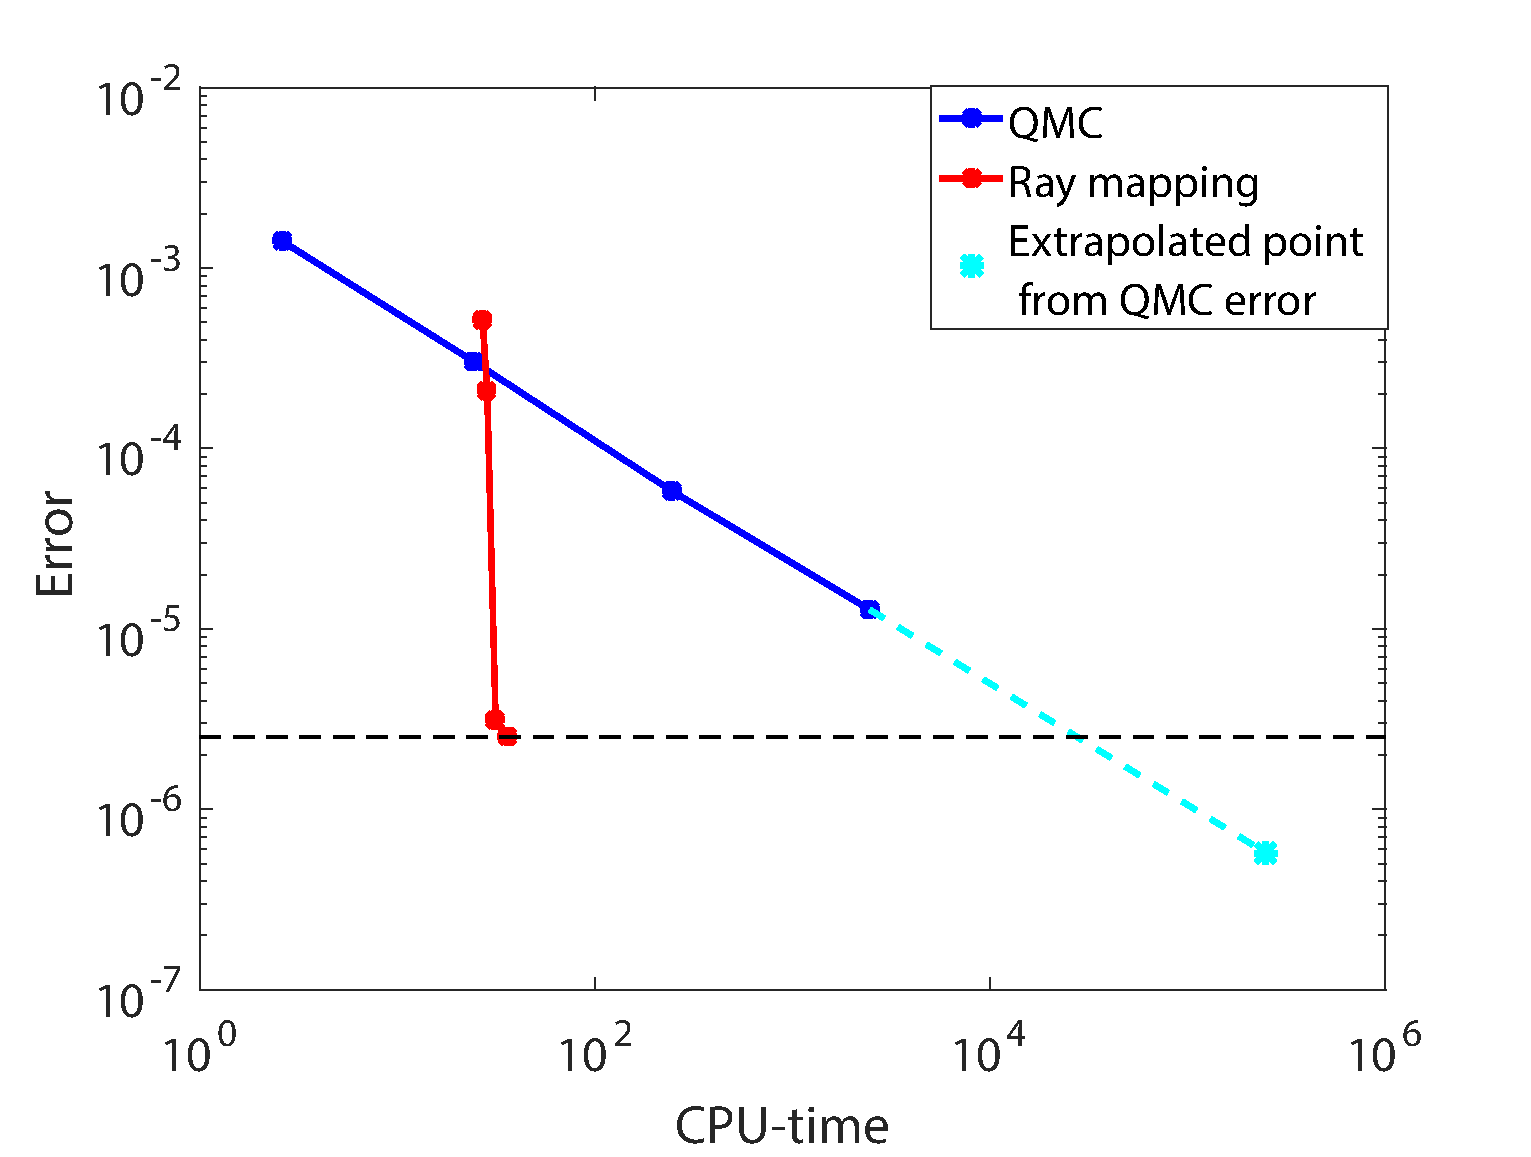
\includegraphics[width=0.7\textwidth]{error_tir_raymapping}
  \end{center}
  \caption{\textbf{Errors of ray mapping and QMC ray tracing for the TIR-collimator.}
 The direct backward ray mapping method is faster and more accurate than QMC ray tracing.}
\label{fig:error_tir_raymapping}
 \end{figure}
In Table \ref{tab:ray_mapping_tir} the numerical results obtained for backward ray mapping are reported. The error values for QMC ray tracing were already reported in Chapter \ref{chap:triangulation} (Table \ref{tab:mc_error_triangulation}).
\begin{table}[t] 
\centering
\caption{\bf Errors of the PS intensity for the TIR-collimator}
\begin{tabular}{llllll}
 \hline  $\textrm{Ni}$\; & $|\Delta U|$  & RM error & CPU-time (sec.)\\
  \hline 
 $5$    & $1.6\cdot 10^{-1}$   & $5.19\cdot10^{-4}$     & $269$  \\
$10$    & $2.8\cdot 10^{-2}$ & $2.09\cdot 10^{-4}$   & $284$   \\
$30$   & $5.7 \cdot 10^{-3}$ & $3.15\cdot 10^{-6}$   & $313$  \\
$100$  & $5.1 \cdot 10^{-3}$ & $2.52\cdot 10^{-6}$   & $359$  \\
 \hline
 \end{tabular}
 \label{tab:ray_mapping_tir}
 \end{table}
\\ \indent In the next section we present the method for a parabolic reflector.
\section{Results for the parabolic reflector}\label{sec:PR}
In this section we provide the results for the parabolic reflector in Figure \ref{fig:PR}.
This is a very challenging example of an optical system. Indeed, the rays that propagate through such a system can reflect many times along the left or the right mirror. As we have seen using PS ray tracing, this leads to many different paths. Every path corresponds to a given number of reflections with one of the two reflectors. In Chapter \ref{chap:triangulation} we found $17$ different paths for this parabolic reflector. Here, we apply the backward ray mapping method to detect all these paths. \\ \indent
The target PS of the parabolic reflector is the rectangular domain \set{T}{}{}$=[-\variabile{b}, \variabile{b}]\times[-1,1]$ where $\variabile{b}=17$. Like for the TIR-collimator, we divide the interval $[-\variabile{b}, \variabile{b}]$ in target PS into sub-intervals of the same length. Considering the partitioning $Q: -\variabile{b}=\variabile{q}^{0}<\variabile{q}^{1}<\cdots<\variabile{q}^{\textrm{Ni}}=\variabile{b}$ of $[-\variabile{b}, \variabile{b}]$ and a direction $\variabile{p}\in[-1,1]$, the backward ray mapping explained in Section \ref{sec:raymapping_explanation} is applied to every sub-interval $[\variabile{q}^{\textrm{k}}, \variabile{q}^{\textrm{k+1}}]\subset[-\variabile{b}, \variabile{b}]$ with $\textrm{k}=0, \cdots, \textrm{Ni}-1$ and for every direction $\variabile{p}\in[-1,1]$. To determine how many bins $\textrm{Ni}$ are needed for a good approximation of the target photometric variables, we employ the same idea of the TIR-collimator. The source \'{e}tendue $U_1$ is compared to several approximations of the \'{e}tendue $U_{\textrm{t}}$ at the target, each of them is given by a different partitioning $Q$ of $[-\variabile{b}, \variabile{b}]$. For the parabolic reflector all the rays emitted from the source arrive at the target. Therefore, the exact \'{e}tendue as an area in PS is computed from (\ref{eq:etenduesource}) obtaining $U=U_1=8$. The approximated target \'{e}tendue $U_{\textrm{t}}$ is given by Equation (\ref{eq:etendueintegraltarget}). In Figure \ref{fig:etendue_ray_mapping_pr_bin} we show the comparison between $U_1$ and several approximations of $U_{\textrm{t}}$ by gradually increasing the number of bins $\textrm{Ni}$ in the partitioning $Q$ while fixing the maximum number of multiple reflections to $30$. Increasing the number of bins $\textrm{Ni}$, $U_{\textrm{t}}$ increases approaching the exact value $U_1=8$. After the division into $\textrm{Ni}=4$ bins the improvement is slightly visible. Therefore, we conclude that $\textrm{Ni}=4$ bins are enough to detect $30$ multiple reflections.
\begin{figure}[t]
  \begin{center}
  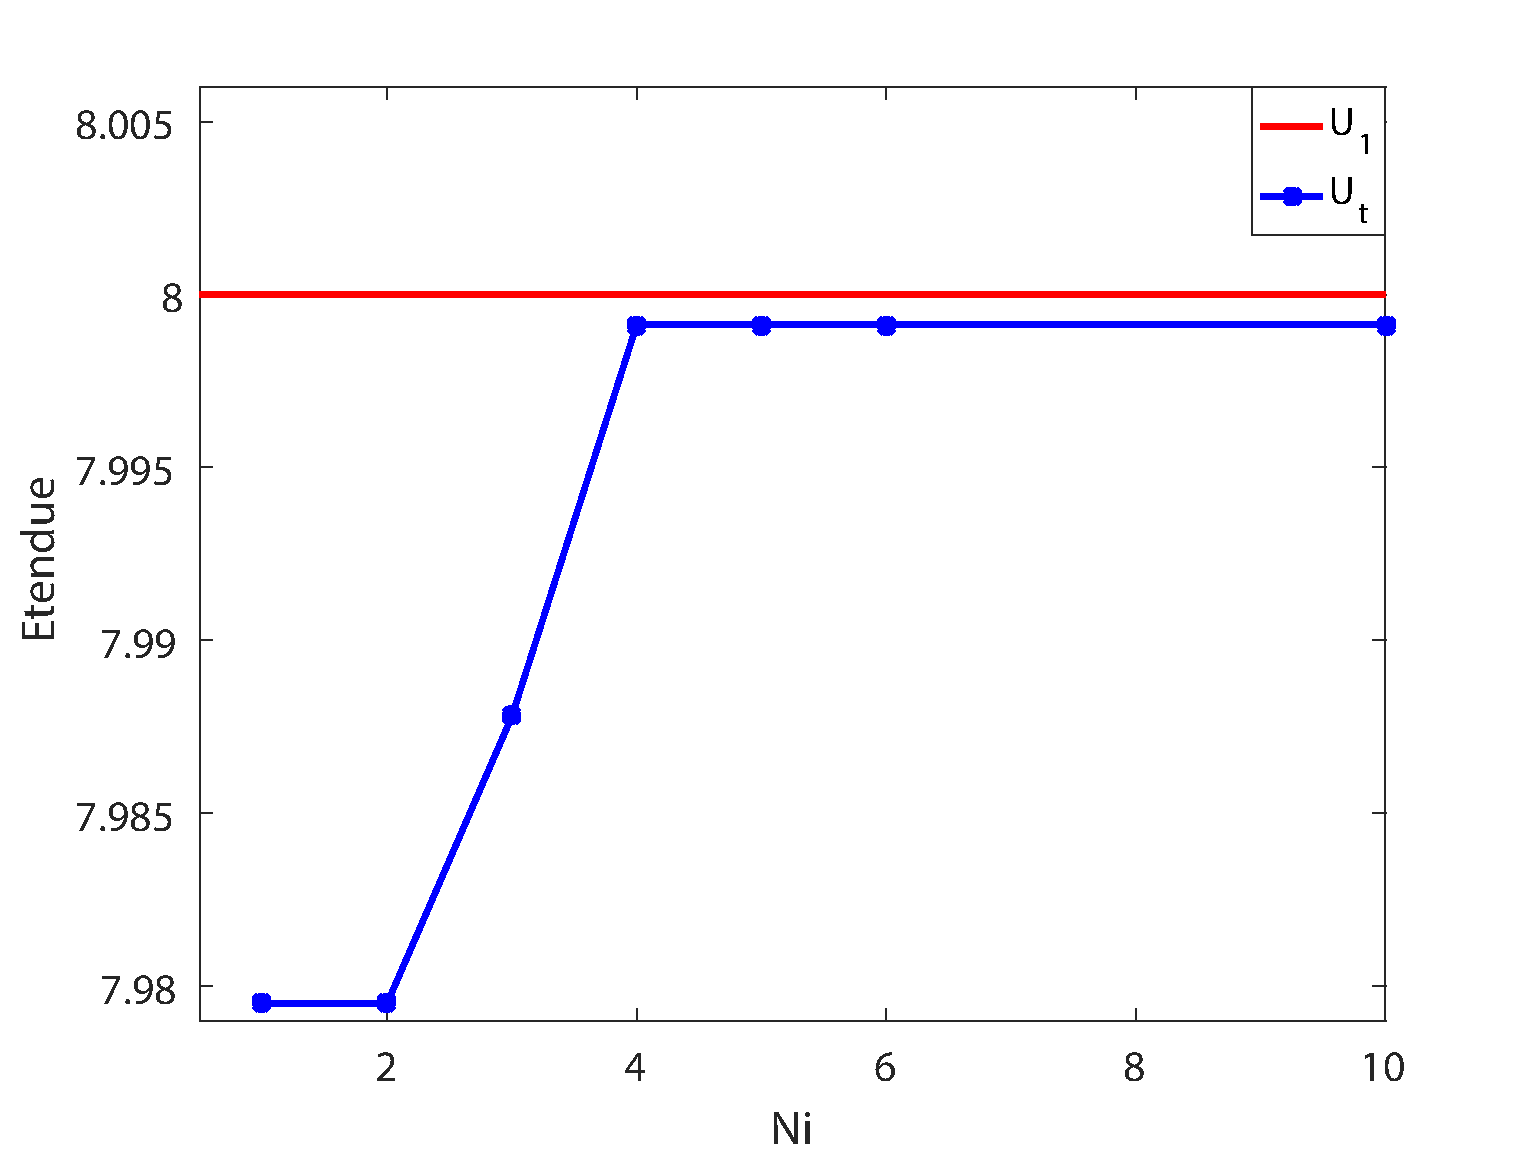
\includegraphics[width=0.7\textwidth]{etendue_ray_mapping_pr_bin}
  \end{center}
  \caption{\textbf{Comparison between the exact \'{e}tendue and the approximated target \'{e}tendue by increasing $\textrm{Ni}$.}
 At most $30$ multiple reflections are considered. Increasing $\textrm{Ni}$, the target \'{e}tendue gets closer to the exact value $U_1=8$.}
\label{fig:etendue_ray_mapping_pr_bin}
 \end{figure}
\\ \indent In Figure \ref{fig:boundaries_rays_pr_raymapping} we show the ray distribution at the target PS obtained using backward ray mapping with $\textrm{Ni}=4$ and at most $30$ multiple reflections. The rays traced from the target to the source are depicted with the red dots. Most of the rays traced are located on the boundaries $\partial$\set{R}{}{}$(\Pi)$ of the regions with positive luminance. 
Only few rays are traced inside those regions. These are the rays located at the end points of every sub-interval $[\variabile{q}^{\textrm{k}}, \variabile{q}^{\textrm{k}+1}]$ with $\textrm{k}=0, \cdots, \textrm{Ni}-1$. 
\begin{figure}[h]
  \begin{center}
  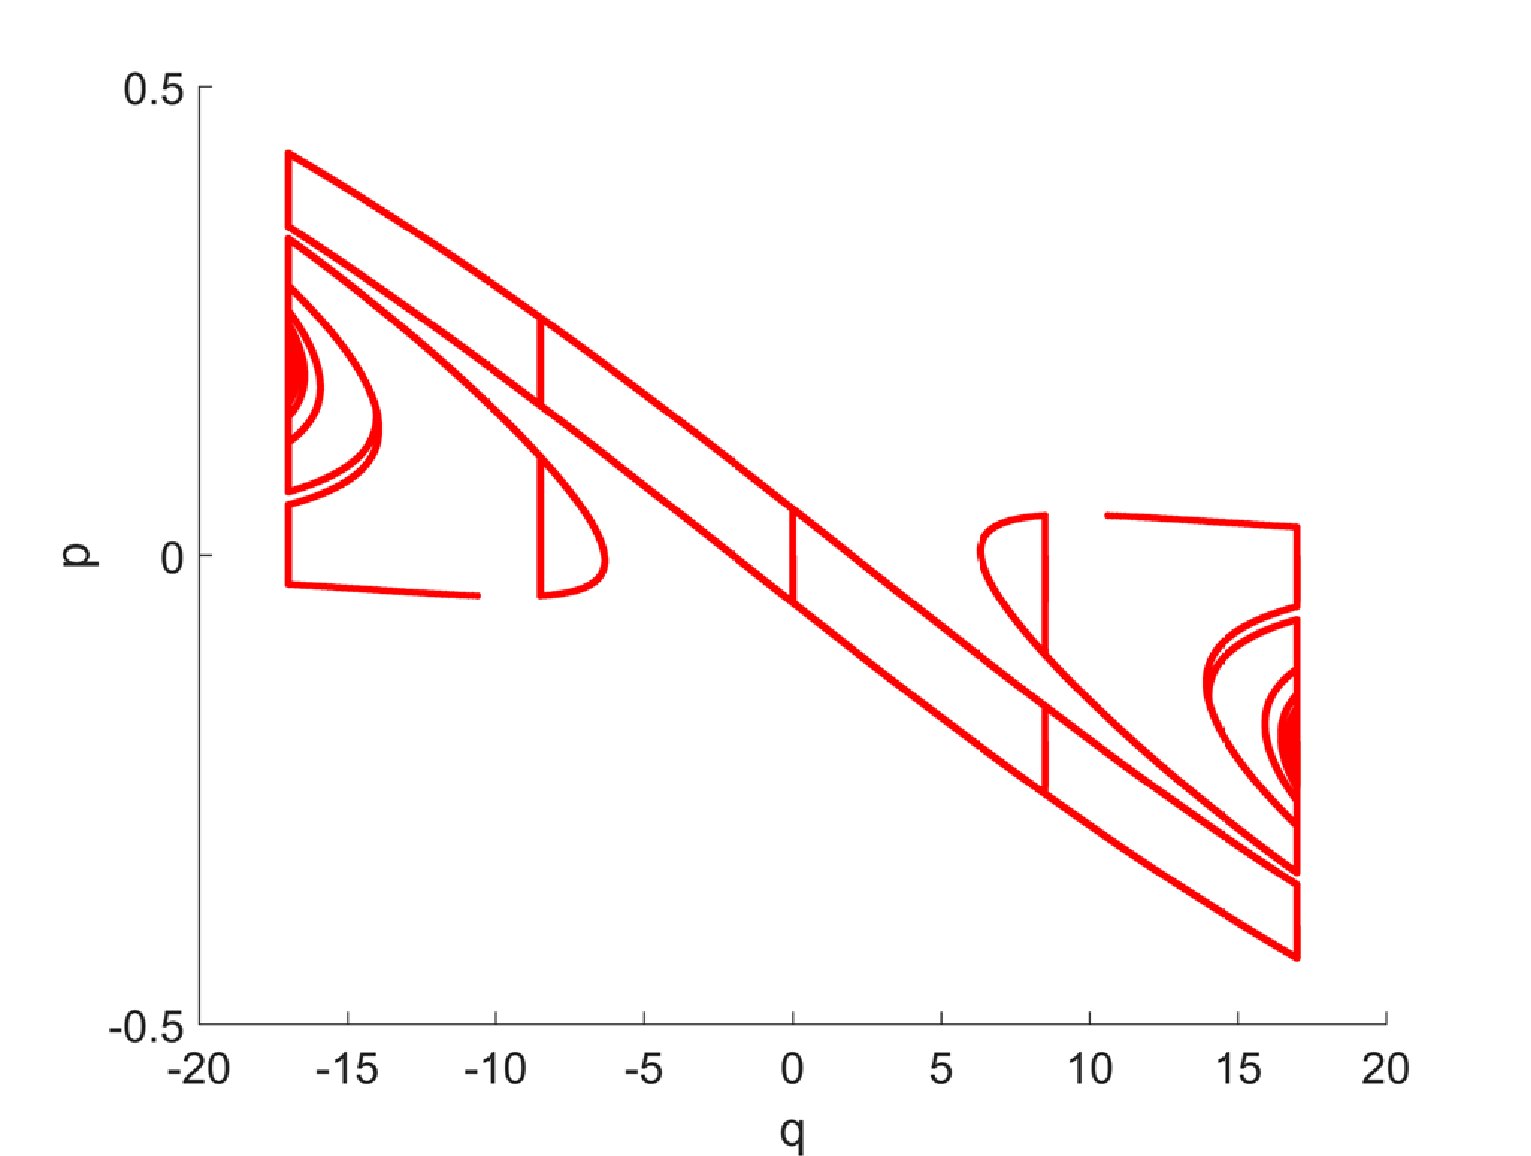
\includegraphics[width=0.7\textwidth]{boundaries_raymapping_pr}
  \end{center}
  \caption{\textbf{Rays on the boundaries of the regions with positive luminance in target PS.}
 At most $30$ multiple reflections are considered and $\textrm{Ni}=4$ and $\nbin = 100$. Only the rays on the boundaries and on the end points of each interval are traced.}
\label{fig:boundaries_rays_pr_raymapping}
 \end{figure}
\\ \indent
The backward ray mapping method is able to detect $61$ different paths. Indeed up to $30$ multiple reflections can occur at the left reflector and the right reflector. The path that goes directly from the source to the target (no reflections) has to be added. Using PS ray tracing we found at most $17$ paths for the same parabolic reflector. Hence, we claim that ray mapping is much more accurate than PS ray tracing. Also, we observe the procedure can be stopped later to detect even more than $30$ reflections. The more reflections are considered the better the accuracy obtained. Again, to define a stopping criterion we use \'{e}tendue conservation. Fixing the number of bins $\textrm{Ni}=4$ and $\nbin=100$ and gradually increasing the number of multiple reflections we see that the approximated target \'{e}tendue $U_{\textrm{t}}$ changes as the blue line in Figure \ref{fig:etendue_pr_raymapping}. The horizontal red line represents the exact intensity $U = U_{1} = 8$. We note that the more reflections are considered the smaller the value of $\Delta U = |U_1-U_{\textrm{t}}|$ (see also Table \ref{tab:ray_mapping_pr}). We observe that after around $30$ multiple reflections there is no significant improvement in the computation of $U_{\textrm{t}}$. This is due to two main reasons. First, since only few rays follow multiple reflections, they do not give a significant contribution to the total \'{e}tendue, the regions in PS formed by those rays are very small compared to the entire PS. Second, when more paths are considered also more bins $\nbin$ and sub-intervals $\textrm{Ni}$ should be taken into account to obtain a more precise approximation of the \'{e}tendue. From this we conclude that backward ray mapping has a good accuracy when around $30$ multiple reflections and $\textrm{Ni}=4$ bins are taken into account.
\begin{figure}[h]
  \begin{center}
  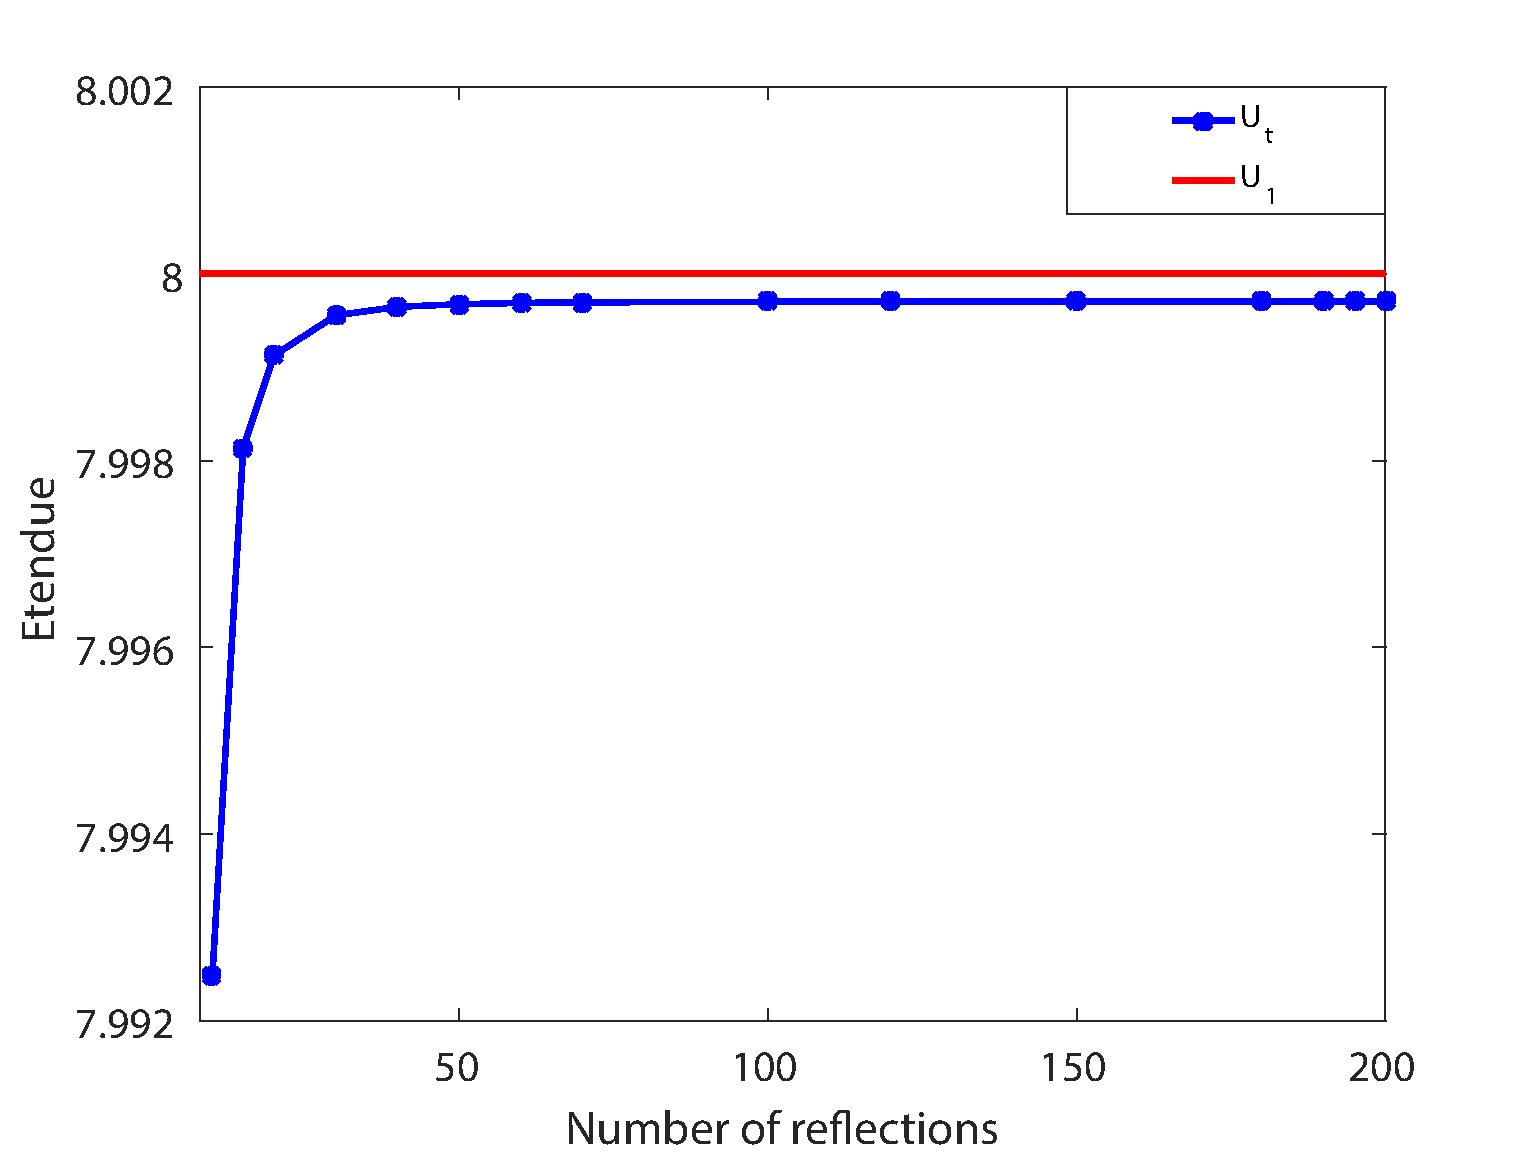
\includegraphics[width=0.7\textwidth]{etendue_pr_raymapping}
  \end{center}
  \caption{\textbf{Comparison between the exact \'{e}tendue and the approximated target \'{e}tendue by increasing the number of multiple reflections.}
Fixing the number of bins along the $\variabile{q}$-axis, $\textrm{Ni}=4$, and increasing the number of reflections considered, the \'{e}tendue increases approaching to the exact value $U_1=8$.}
\label{fig:etendue_pr_raymapping}
 \end{figure}
Once a stopping criterion is established, ray mapping is run and the rays on the boundaries are determined. Finally, the target intensity is calculated from Equation (\ref{eta2}). 
\\ \indent In Figure \ref{fig:intensity_pr_raymapping} both the ray mapping intensity (red line) and the reference intensity (dotted blue line) are shown. The ray mapping intensity $\hat{I}_{\textrm{RM}}$ is obtained considering at most $30$ multiple reflections, $\textrm{Ni}=4$ and $\nbin = 100$. The reference intensity $\hat{I}_{\textrm{ref}}$ is given by QMC ray tracing with $10^8$ rays and $\nbin = 100$. The two intensities coincide.
\begin{figure}[t]
  \begin{center}
  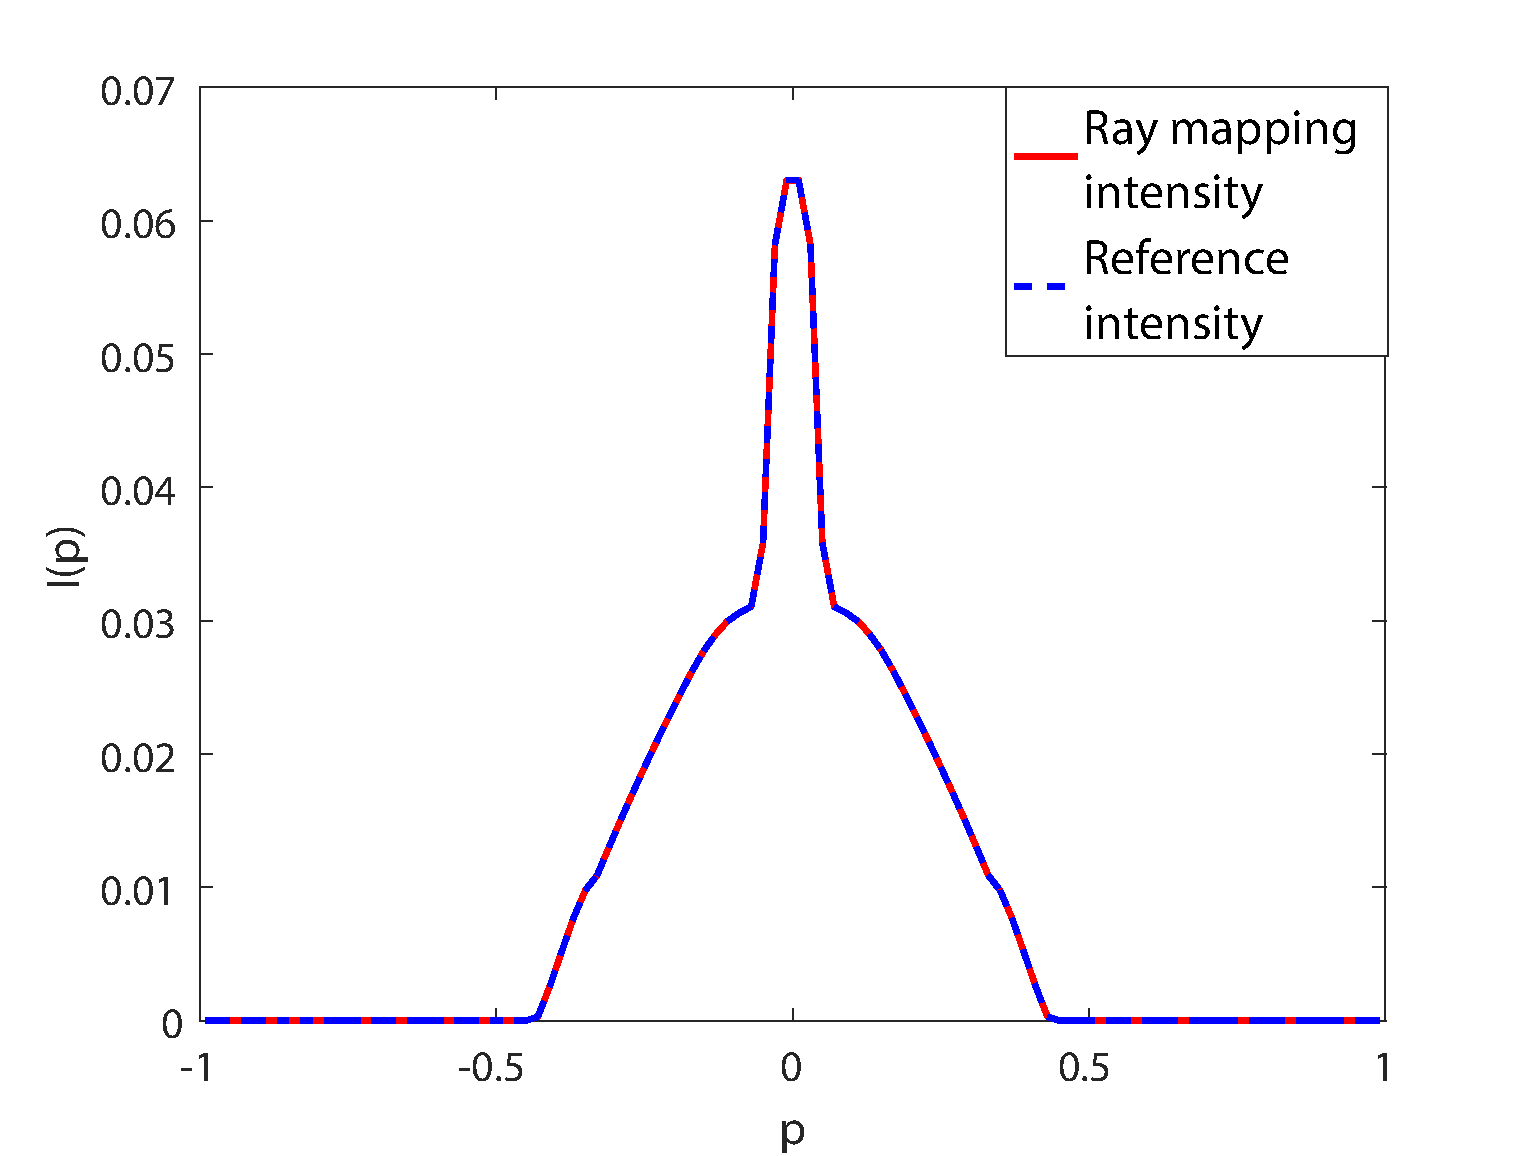
\includegraphics[width=0.7\textwidth]{intensity_pr_raymapping}
  \end{center}
  \caption{\textbf{Ray mapping intensity compared to a reference intensity.}
The ray mapping error is calculated considering $\textrm{Ni}=4$ and at most $30$ multiple reflections. The reference intensity is obtained by running QMC ray tracing with $10^8$ rays.}
\label{fig:intensity_pr_raymapping}
 \end{figure}
\\ \indent
To conclude, we calculate the errors between the approximated intensity $\hat{I}_{\textrm{A}} (\textrm{A}=\textrm{RM}, \textrm{QMC})$ and the reference intensity $\hat{I}_{\textrm{ref}}$. From the results in Figure \ref{fig:error_raymapping_pr} we observe that the RM error (red line) converges faster than the QMC error (blues line) as long as an error of an order of $10^{-6}$ is desired. Ray mapping results to be around $1000$ times faster than QMC ray tracing! Furthermore, it is much more accurate than QMC. Our method is able to detect \textit{all} the possible paths that can occur. The procedure is stopped when $200$ multiple reflections are reached. Our expectation is that, increasing the number of multiple reflections and the number of bins $\textrm{Ni}$, the accuracy can be improved even more.
\begin{figure}[h]
  \begin{center}
  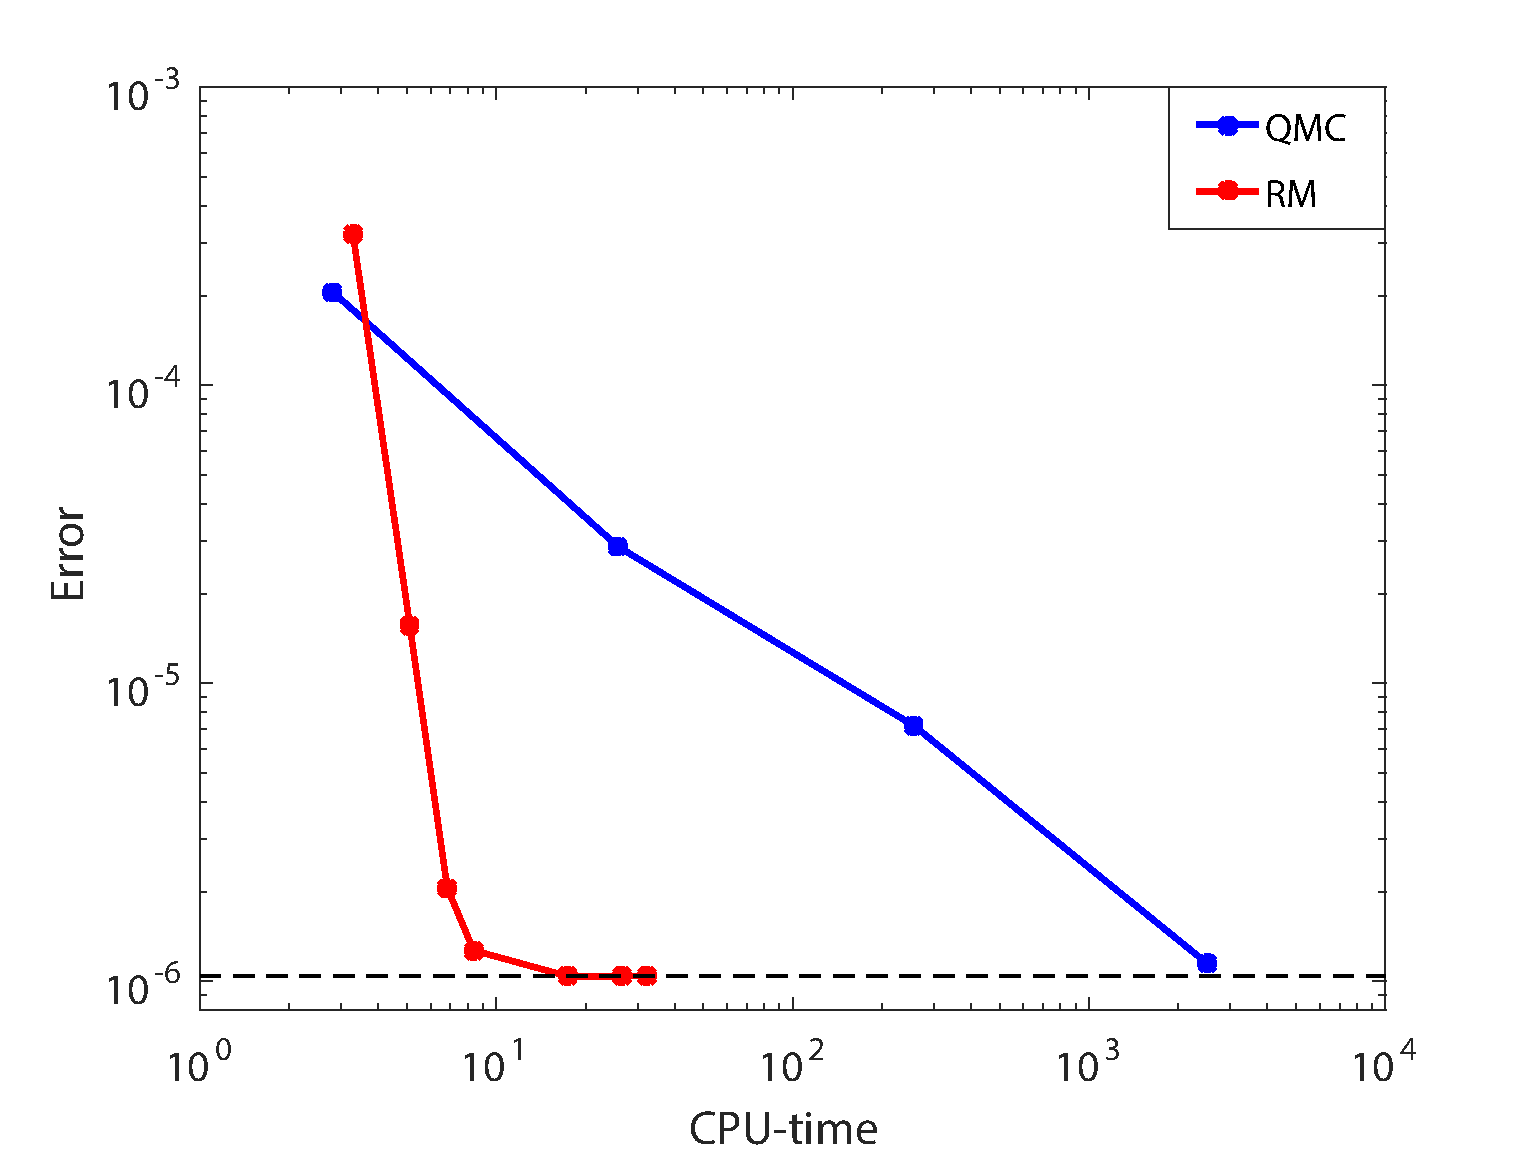
\includegraphics[width=0.7\textwidth]{error_pr_raymapping}
  \end{center}
  \caption{\textbf{Errors of ray mapping and QMC ray tracing for the parabolic reflector.}
The ray mapping error decreases by increasing the number of reflections considered.
The QMC error reduces by tracing more rays.
 The extended backward ray mapping method is significantly faster and more accurate than QMC ray tracing.}
\label{fig:error_raymapping_pr}
 \end{figure}
In Tables \ref{tab:ray_mapping_pr} and \ref{tab:qmc_raymapping_pr} these numerical results are reported.
\begin{table}[t] 
\centering
\caption{\bf Errors of the ray mapping intensity for the parabolic reflector}
\begin{tabular}{llllll}
 \hline  Number of\\
 reflections\;  & $|\Delta U|$ & RM error  & CPU-time (sec.)\\
  \hline 
 $5$      & $1.74\cdot 10^{-1}$  & $3.222\cdot10^{-4}$& $3.28$  \\
$10$      & $7.52\cdot 10^{-3}$ & $1.555\cdot 10^{-5}$& $5.11$   \\
$20$      & $9.00 \cdot 10^{-4}$ & $2.059\cdot 10^{-6}$& $6.83$  \\
 $30$    & $5.00 \cdot 10^{-4}$ & $1.269\cdot 10^{-6}$ & $8.38$  \\
$100$    & $2.99 \cdot 10^{-4}$ & $1.038\cdot 10^{-6}$ & $17.49$  \\
$150$    & $2.96 \cdot 10^{-4}$ & $1.039\cdot 10^{-6}$ & $26.38$  \\
$200$    & $2.95 \cdot 10^{-4}$ & $1.039\cdot 10^{-6}$ & $32.21$  \\
 \hline
 \end{tabular}
 \label{tab:ray_mapping_pr}
 \end{table}
\begin{table}[t] 
\centering
\caption{\bf Errors of the QMC intensity for the parabolic reflector}
\begin{tabular}{lllll}
 \hline  $\nrays$\;  & QMC error & CPU-time (sec.)\\
  \hline 
$10^4$     & $2.05\cdot 10^{-4}$   & $2.81$  \\
$10^5$     & $2.87\cdot 10^{-5}$   & $25.81$   \\
$10^6$     & $7.18 \cdot 10^{-6}$  & $257.54$  \\
$10^7$     & $1.15 \cdot 10^{-6}$  & $2491.32$  \\
 \hline
 \end{tabular}
 \label{tab:qmc_raymapping_pr}
 \end{table}
\section{Conclusions}
In this chapter we extended the concateneted ray mapping method to systems formed by curved lines. Employing backward ray tracing and a bisection procedure in target PS, an inverse map from the target to the source was constructed such that all the possible paths that the rays can follow are determined. The numerical backward ray mapping method is able to detect the rays located on the boundaries of the regions formed by rays that follow the same path. From these rays the target intensity is calculated. 
\\ \indent
We presented two examples of optical systems: the TIR-collimator and the parabolic reflector. In both cases the target PS is divided into bins and the procedure is applied to each bin. A stopping criterion based on \'{e}tendue conservation is developed to determine the number of bins needed to obtain a good accuracy. For the TIR-collimator we noticed that the method is able to detect rays that follow a spurious path due to numerical error. This gives the expectation that backward ray mapping can be used for detecting stray light.
For the parabolic reflector, many paths can occur along the reflectors. Etendue conservation is used again to determine the number of multiple reflections to be considered. The target intensity is computed for both systems and is compared with a reference intensity given by QMC ray tracing with a large number of rays. The results show that the method is able to detect all the possible paths tracing a relatively small number of rays, typically around $10^3$. Comparing our method to QMC ray tracing, significant advantages are observed in accuracy and computational time for both optical systems.
% Explain the results
\\ \indent In the next chapter we explain how to apply the method to systems with Fresnel reflection. We present the method for a system formed by the source, an ideal lens and the target. 













